% ============================================================
%  Tactical Formation — English edition
%  Entry point — only \input the modules
%  Compile: xelatex main && bibtex main && xelatex main && xelatex main
% ============================================================

% !TeX root = main.tex
% ============================================================
%  Tactical Formation — Preamble (English edition)
%  Compile (XeLaTeX, default):
%    xelatex main && bibtex main && xelatex main && xelatex main
%  To use pdfLaTeX: the iftex block below falls back automatically.
% ============================================================

\documentclass[12pt, a4paper]{article}

% ── Encoding & Language (auto-detect engine) ─────────────────
% Auto-detects the compiler: runs under BOTH pdfLaTeX (Overleaf
% default) and XeLaTeX/LuaLaTeX. T5 font encoding is kept on the
% pdfLaTeX path so the author's Vietnamese name still renders.
\usepackage{iftex}
\ifPDFTeX
  % pdfLaTeX
  \usepackage[utf8]{inputenc}
  \usepackage[T5]{fontenc}
  \usepackage{lmodern}
  \usepackage[english]{babel}
\else
  % XeLaTeX / LuaLaTeX
  \usepackage{fontspec}
  \usepackage{polyglossia}
  \setdefaultlanguage{english}
  % Latin Modern carries the Vietnamese diacritics in the author
  % name; swap to `TeX Gyre Termes` or `Noto Serif` if glyphs miss.
  \setmainfont{Latin Modern Roman}
\fi

% ── Page Layout ──────────────────────────────────────────────
\usepackage[top=2.5cm, bottom=2.5cm, left=2.5cm, right=2.5cm]{geometry}

% ── Math ─────────────────────────────────────────────────────
\usepackage{amsmath, amssymb}

% ── Tables ───────────────────────────────────────────────────
\usepackage{booktabs}
\usepackage{tabularx}
\usepackage{array}

% ── Graphics & Diagrams ──────────────────────────────────────
\usepackage{tikz}
\usetikzlibrary{arrows.meta, positioning, shapes.geometric}
\usepackage{graphicx}
\usepackage{float}

% ── Colors ───────────────────────────────────────────────────
\usepackage{xcolor}
\definecolor{vertexcolor}{RGB}{50,  100, 200}
\definecolor{centercolor}{RGB}{200, 80,  50}
\definecolor{yellowpiece}{RGB}{240, 200, 0}
\definecolor{greenpiece} {RGB}{50,  180, 80}

% ── Author / Affiliation ─────────────────────────────────────
\usepackage{authblk}

% ── Bibliography (APA 7 via natbib) ──────────────────────────
\usepackage[round]{natbib}
\bibliographystyle{apalike}

% ── Hyperlinks ───────────────────────────────────────────────
\usepackage{hyperref}
\usepackage{xurl}            % allow line breaks inside long URLs
\hypersetup{
  colorlinks = true,
  linkcolor  = blue,
  urlcolor   = blue,
  citecolor  = blue,
  pdftitle   = {Cờ Trận (Tactical Formation): Documenting and Analysing a Vietnamese Folk Board Game for 2–4 Players},
  pdfauthor  = {Trương Văn Quyết},
  pdfkeywords = {Vietnamese folk game, traditional board game, intangible cultural heritage, Paranoid Minimax}
}

% ── Pseudocode ───────────────────────────────────────────────
\usepackage{algorithm}
\usepackage{algpseudocode}

% ── Code Listings ────────────────────────────────────────────
\usepackage{listings}
\lstset{basicstyle=\ttfamily\small, breaklines=true,
        frame=single, captionpos=b}

% ── Misc ─────────────────────────────────────────────────────
\usepackage{enumitem}
\usepackage{caption}
\usepackage{subcaption}
\usepackage{setspace}
\onehalfspacing

% English words are longer than Vietnamese syllables, so a few lines with
% unbreakable \texttt{} filenames or math coordinate runs would otherwise
% poke into the margin. A last-resort stretch absorbs the slack without
% altering any content.
\emergencystretch=3em

% (Board figures are screenshots from the game — see
%  tools/make_figures.py; the hand-drawn TikZ macros are no longer used.)


% ── Title block ──────────────────────────────────────────────
\title{%
  \textbf{Cờ Trận (Tactical Formation):}\\[0.3em]
  \textbf{Documenting and Analysing}\\[0.3em]
  \textbf{a Vietnamese Folk Board Game}\\[0.3em]
  \textbf{for 2--4 Players}
}
\author{%
  Trương Văn Quyết%
  \thanks{Corresponding author: \href{mailto:quyetops@gmail.com}{quyetops@gmail.com}}
}
\affil{Independent Researcher, Vietnam}
\date{Preprint, version 1 \,·\, October 2026\\[0.3em]
  \href{https://doi.org/10.5281/zenodo.23437472}{doi:10.5281/zenodo.23437472}}

% ─────────────────────────────────────────────────────────────
\begin{document}
% ─────────────────────────────────────────────────────────────

\maketitle

% !TeX root = ../main.tex
% ─────────────────────────────────────────────────────────────
%  Abstract — English edition. 150–300 words answering the four
%  questions: problem / what we did / results / significance.
% ─────────────────────────────────────────────────────────────

\begin{abstract}
% (1) Problem
Many Vietnamese folk board games survive only by word of mouth among village
children, and they are slowly being forgotten. \textbf{Cờ Trận} is one such
game. It was played in Đồng Bùa hamlet, Tam Quan commune, Tam Đảo district,
Vĩnh Phúc province, using whatever could be picked up by the roadside as
pieces: stones, pebbles, twigs, leaves. To our knowledge it has never been
written down.
% (2) What we did
This paper records the complete rules of Cờ Trận for two, three and four
players, from the recollection of the author, who played it throughout
grades 5 to 9. We refer to it in English as \emph{Tactical Formation}. A
piece moves by jumping over an adjacent piece of any side, and the
jumped-over piece stays on the board. After landing, the moving piece
sandwiches the line of enemy pieces lying between it and a friendly piece,
and that whole line changes side. The board has two layers of positions,
vertices and centres: a vertex piece moves in 8 directions and a centre
piece in 4.
% (3) Results
We give a formal mathematical model of the two-player mode, stating a
\emph{28-piece conservation law} (capture $=$ change of side, never
removal). We also implement the game as open-source software, with an AI
based on Minimax search with Alpha-Beta pruning (the Paranoid variant for the
multiplayer modes). Experiments measure the branching factor and the think
time per move, and a two-player bot-vs-bot tournament shows that deeper
search wins consistently.
% (4) Significance
Through a written record, a formal model and software that anyone can play,
the paper helps keep a folk game from disappearing entirely.
\end{abstract}

\vspace{0.4em}
\noindent\textbf{Keywords:}
Vietnamese folk game;
traditional board game;
intangible cultural heritage;
abstract board game;
Paranoid Minimax;
multiplayer board game.


\vspace{0.8em}
\hrule
\vspace{0.4em}

\tableofcontents
\newpage

% !TeX root = ../main.tex
\section{Introduction}
\label{sec:intro}

Folk games are part of intangible cultural heritage, which the UNESCO
Convention describes as \emph{transmitted from generation to
generation}~\citep{unesco2003ich}. Many Vietnamese folk board games have no
written rules; the rules are kept only in the memory of the people who
played them. When those players grow up and stop playing, a game can vanish
without a trace. Some games have been recorded
and digitised, such as Shoulder-Pole Chess (our translation of its Vietnamese name) from
Quang Nam~\citep{mytour_coganh}. Many
others have not.

\textbf{Tactical Formation} belongs to the second group. It is a board game
played by the children of Dong Bua hamlet, Tam Quan commune, Tam Dao
district, Vinh Phuc province; \emph{Tactical Formation} is the author's
English rendering of its village name (Section~\ref{sec:provenance}). The
author played the game throughout grades 5 to 9. Today almost nobody in the village remembers
the game, and the author had partly forgotten it too. This paper comes from
the wish to keep Tactical Formation from being forgotten: to write its rules down, to
model it mathematically, and to put it into software that anyone can play.
The author did \emph{not} create Tactical Formation and does not know who did.
Section~\ref{sec:provenance} describes its origin and how it was recorded.

In terms of mechanics, every move in Tactical Formation is a \emph{jump} over an
adjacent piece, including one's own. The jumped-over piece stays on the
board. From the landing square, the player \emph{sandwiches} the line of
enemy pieces lying between the moved piece and a friendly piece, and that
whole line changes side. Every move therefore has two effects at once: the
new position of the piece shapes future jumps, and the sandwich formed from
that position flips pieces immediately. The player must weigh both. Taken
one at a time, the jump resembles Halma and the capture resembles Reversi.
Section~\ref{sec:related} compares Tactical Formation with these games in detail.

The paper makes the following contributions:
\begin{enumerate}[label=(\roman*)]
  \item To our knowledge, the first complete and consistent written record
        of the rules of Tactical Formation for 2--4 players, together with a record of
        the game's origin. The 3-player starting configuration is recorded
        exactly as in the folk game, even though it is unbalanced; see
        Section~\ref{sec:limitations}.
  \item A description of the two-layer board structure (vertices and
        centres), with the movement and capture directions of each kind of piece.
  \item A formal mathematical model for the 2-player mode, together with
        the 28-piece conservation invariant (\emph{capture = change of
        side}) and upper bounds on the number of actions and states.
  \item A companion AI based on Minimax and Paranoid Minimax, with the
        reasons for not using MCTS.
  \item An empirical evaluation of the game and the AI via branching
        factor and game length (2--4 players), games between bots (2-player
        mode), and the bots' think time.
  \item An open-source software release, as a form of digitisation and
        preservation, so that the community can play and study the game.
\end{enumerate}

The remainder of the paper is organised as follows.
Section~\ref{sec:provenance} describes the origin of the game and the
recording method. Section~\ref{sec:related} compares Tactical Formation with related
games. Section~\ref{sec:rules} gives a complete specification of the rules
through board images. Section~\ref{sec:variants} describes the multiplayer
modes. Section~\ref{sec:ai} presents the companion-AI algorithm.
Section~\ref{sec:impl} describes the software. Section~\ref{sec:eval}
gives the empirical evaluation. Section~\ref{sec:limitations} states the
limitations, and Section~\ref{sec:conclusion} concludes. The full formal
mathematical model for the 2-player mode is presented in
Appendix~\ref{app:formal}.

% !TeX root = ../main.tex
% ─────────────────────────────────────────────────────────────
%  PROVENANCE — Cờ Trận is a folk game; the author did NOT create it.
%  Everything here comes from the author's recollection (14 Oct 2026).
% ─────────────────────────────────────────────────────────────
\section{Origin and Recording Method}
\label{sec:provenance}

\subsection{Place, players and name}

Cờ Trận was a children's game in Đồng Bùa hamlet, Tam Quan commune, Tam Đảo
district, Vĩnh Phúc province, Vietnam. We use the place names of the
administrative boundaries at the time the game was played; since 2025,
Vĩnh Phúc province has been merged into Phú Thọ province. The author was
taught Cờ Trận in grade 5, around the 2011--2012 school year, and played it
with friends in the village until the end of grade 9, around 2016, and then
stopped. The game was thus passed on to the author by earlier players; it
did not start with the author's generation.

A four-player game usually lasted three to four hours, from midday until
the evening. The folk game has \emph{no} move limit: a game ends only by the
winning conditions in Section~\ref{sec:rules}.

``Cờ Trận'' is the name used in the village. \emph{Cờ} means a board game,
and \emph{trận} evokes a battle or a battle formation. The English name
\emph{Tactical Formation} is the author's rendering of this name for an
international readership; it is not a folk name.

\subsection{Board and pieces}

The game needs no manufactured equipment. The board was drawn directly on the
road. On a dirt road, players scratched it into the ground with a
stick; on a concrete road, they drew it with a stone, chalk or a piece of
brick so that the lines would last longer. Pieces were whatever could be
picked up by the roadside: stones, pebbles, dry or green twigs, leaves.
Each side used a different kind of object. To capture, a player removed the
captured side's object and put one of their own in exactly that spot. This
keeps the total number of pieces on the board unchanged, matching the
conservation invariant in Appendix~\ref{app:formal}. Using found objects also
explains why the game has left no physical artefacts behind.

\subsection{Recording method and reliability}

The rules in this paper were written down from the author's own
recollection. According to the author, the record is complete and faithful
to the folk game in all of the following: the two-layer vertex--centre
board, the jump move, the sandwich rule and the choice of a single capture
direction, the number of pieces and the starting layout, the winning
condition, and all three modes for 2, 3 and 4 players.

We have not yet been able to check this record against a second source.
Most people in the village have forgotten the game. Web searches in
Vietnamese and English (October 2026) found no document describing Cờ Trận
or any game with the same rule set. The record therefore rests on \emph{a
single informant}, a limitation we state explicitly in
Section~\ref{sec:limitations}. We invite anyone who knows Cờ Trận, or a
variant of it from another village, to contact the author so that the
record can be extended and cross-checked.

\subsection{What is folk tradition and what was added}

So that readers do not confuse the folk game with the contributions of this
paper, we separate the two clearly:
\begin{itemize}
  \item \textbf{Part of the folk game}: all the rules specified in
        Sections~\ref{sec:rules} and~\ref{sec:variants}.
  \item \textbf{Added by the author}: the English name; the formal
        mathematical model (Appendix~\ref{app:formal}); the software and
        interface (Section~\ref{sec:impl}); the fixed turn order in the
        software (Section~\ref{ssec:turn_order}); the entire AI
        (Section~\ref{sec:ai}); and the experiments
        (Section~\ref{sec:eval}).
\end{itemize}

% !TeX root = ../main.tex
\section{Related Games}
\label{sec:related}

Tactical Formation is a folk game, not a game designed on the basis of the games
below. We compare them in order to situate its mechanics, without claiming
any historical relationship between the games. Folk games in different
places often share mechanics with one another.

\subsection{Games with a jump move}

In Checkers~\citep{schaeffer2007checkers}, a piece jumps over an
\emph{opponent's} piece to capture it, and the jumped-over piece is removed
from the board. In Halma and its relative Chinese Checkers, a piece may jump
over \emph{any} adjacent piece, its own or an opponent's, and the jumped-over
piece is \emph{not} removed~\citep{britannica_halma}. Chinese Checkers is
played by several players and has served as a test domain for multi-player
search algorithms~\citep{nijssen2013mcts}. The jump in Tactical Formation matches Halma
on both of these points. The differences are that Tactical Formation allows
\emph{only} jumps (there is no single step into an adjacent square), a turn
contains a single jump, and the jump triggers the sandwich-flip rule. Halma
has no capture at all.

\subsection{Games that capture by conversion}

In Reversi/Othello, a player \emph{places a new piece} and flips every
opponent piece sandwiched in a straight line, in \emph{all} directions at
once. The Logistello program of \citet{buro1997othello} once defeated the
world champion, and Othello $8\times8$ has recently been proven a
\emph{draw} under optimal play by both sides~\citep{takizawa2023othello}.
Rolit is a Reversi variant for up to 4 players, and it has been used as a
test domain for Paranoid, max$^n$ and Best-Reply
Search~\citep{schadd2011brs,nijssen2013mcts}. The
Reversi-like class of sandwich-flip games therefore already has a
multiplayer version. The sandwich rule of Tactical Formation is close to Reversi, with
three differences: pieces are \emph{moved} rather than placed; when several
sandwich lines are available, the mover takes only \emph{one}; and the total
number of pieces never changes.

The idea that ``capture is a change of side and the piece count is
conserved'' is not new either. In \emph{Shoulder-Pole Chess} from Quang Nam, a piece
steps along the lines of a 25-point board. If it moves into the point
between two enemy pieces in a straight line, those two pieces change side
(capture by \emph{intervention}: the moving piece ``carries'' the pair like a
shoulder pole, which gives the game its name), and a piece surrounded until it has no move also changes
side~\citep{mytour_coganh,fptshop_coganh}. The capture geometry of Shoulder-Pole Chess
is the reverse of Tactical Formation: in Shoulder-Pole Chess one's own piece moves \emph{between}
two enemy pieces, whereas in Tactical Formation enemy pieces are caught \emph{between}
two of one's own. In \emph{Ming Mang} (Tibet), pieces slide in straight lines
like a rook, and a line of enemy pieces sandwiched in a straight line passes
to the capturing side~\citep{wiki_mingmang}. This is the closest precedent
for the sandwich-conversion of Tactical Formation. \emph{Ataxx} also has a jump move,
after which every enemy piece \emph{adjacent} to the landing square changes
side, not along a line; its one-step move creates a new piece, so the total
piece count grows~\citep{gebop_ataxx}.

\subsection{Other piece-moving games}

\emph{Lines of Action}, designed by Claude Soucie and described in the
collection of \citet{sackson1969gamut}, also moves existing pieces instead
of placing new ones; the winning objective is to connect one's pieces, and
a captured piece is still removed from the board, as in Checkers. \emph{Focus} (also called \emph{Domination}) by
Sid Sackson~\citep{sackson1969gamut} keeps captured pieces so that they can
return to the board, so it too treats capture as transformation rather than
removal.

\subsection{Recording and digitising traditional games}

The Ludii system~\citep{piette2020ludii} describes board games, including
many traditional games, in a common game description language, so that
machines can play and compare them. This paper follows the same spirit: it
records a traditional game, models it, and implements it in order to
preserve it. Adding Tactical Formation to Ludii is a natural next step
(Section~\ref{sec:conclusion}).

\subsection{Overview comparison}

Table~\ref{tab:comparison} summarises the similarities and differences. To
our knowledge, no recorded game has all five of the following features of
Tactical Formation at once: (1)~movement only by jumping over any piece, with the
jumped-over piece staying in place; (2)~sandwich capture along a straight
line that converts pieces, but in a single chosen direction; (3)~a
two-layer vertex--centre board, with 8 directions for vertex pieces and 4
for centre pieces; (4)~a constant total number of pieces; (5)~play for 2 to
4 players. Each feature on its own already appears in other games.

\begin{table}[H]
  \centering
  \caption{Comparison of Tactical Formation with related games.}
  \label{tab:comparison}
  \footnotesize
  \renewcommand{\arraystretch}{1.2}
  \begin{tabularx}{\linewidth}{l*{6}{>{\centering\arraybackslash}X}}
    \toprule
    \textbf{Feature} & \textbf{Checkers} & \textbf{Halma / Chinese Checkers}
      & \textbf{Reversi / Rolit} & \textbf{Shoulder-Pole Chess} & \textbf{Ming Mang}
      & \textbf{Tactical Formation} \\
    \midrule
    Movement         & Diagonal step, jump & Step or jump & Place new piece
                     & Single step & Rook-like slide & Jump only \\
    Jumps over       & Enemy piece & Any piece & --- & --- & --- & Any piece \\
    Jumped-over piece & Removed & Stays & --- & --- & --- & Stays \\
    Capture          & Jump & None & Sandwich, all directions
                     & Inter\-vention, surround & Sandwich & Sandwich, one direction \\
    Captured piece   & Removed & --- & Changes side & Changes side
                     & Changes side & Changes side \\
    Total pieces     & Decreases & Constant & Increases & Constant & Constant
                     & Constant \\
    Players          & 2 & 2--6 & 2 / 2--4 & 2 & 2 & 2--4 \\
    Position layers  & 1 & 1 & 1 & 1 & 1 & 2 (vertex + centre) \\
    \bottomrule
  \end{tabularx}
\end{table}

% !TeX root = ../main.tex
\section{The Rules Through Images}
\label{sec:rules}

This section presents the rules through \emph{screenshots of the software}
rather than formulas, enough for a
non-mathematical reader to grasp the whole game; the corresponding formal
mathematical specification (2-player mode) is in
Appendix~\ref{app:formal}. Convention: \textbf{Green} pieces are drawn in
green and \textbf{Yellow} pieces in yellow; \emph{vertex} pieces sit on the
intersections of the square grid, while \emph{centre} pieces sit between
four vertices. All markers in the images are drawn by the software: a
\emph{yellow ring} marks the selected piece, \emph{green dots} are the
valid landing cells, and \emph{yellow lines} indicate the sandwich ray
from the landing cell. The notation $\mathrm G@(x,y)$ denotes a Green piece
on cell $(x,y)$, and $\mathrm Y@(x,y)$ a Yellow piece.

\subsection{The board---41 cells on two layers}
\label{ssec:vis_board}

\begin{figure}[H]
  \centering
  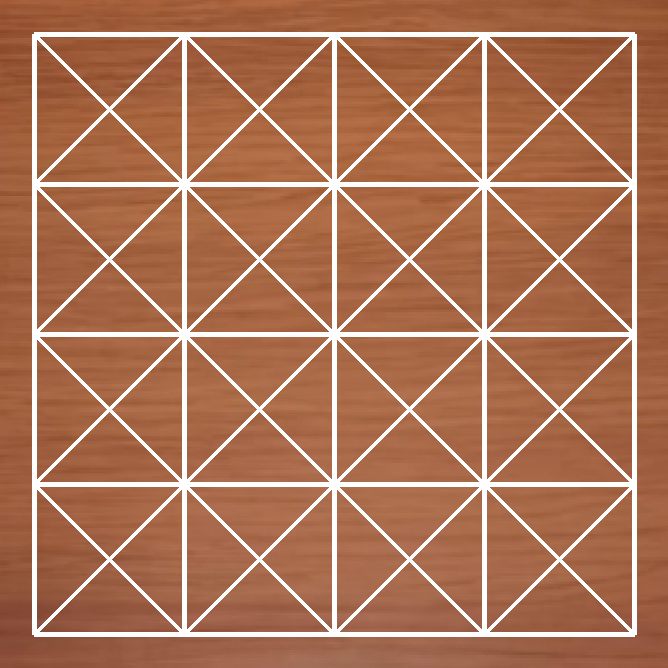
\includegraphics[width=0.5\linewidth]{figures/board_2p_empty.png}
  \caption{Structure of the 2-player board (screenshot of the software,
  the game): 25 \textbf{vertex} cells (intersections of the square grid,
  with integer coordinates such as $(0,0),(2,3)$) plus 16 \textbf{centre}
  cells (intersections of the diagonals, with half-integer coordinates such
  as $(0.5,0.5)$), each centre cell lying exactly in the middle of four
  vertex cells. 41 cells in total. Vertex and centre pieces operate on two
  separate layers that interlock through the diagonals.}
  \label{fig:board41}
\end{figure}

\begin{table}[H]
  \centering
  \caption{Board size and configuration by game mode (exact coordinates and
  starting positions for 3--4 players in
  Appendix~\ref{app:multistart}).}
  \label{tab:board_size}
  \begin{tabular}{lcccc}
    \toprule
    \textbf{Mode} & \textbf{Size} & \textbf{Coordinates}
    & \textbf{Removed cells} & \textbf{Pieces/player} \\
    \midrule
    2-player & 5{\texttimes}5 vertex & $0\text{--}4 \times 0\text{--}4$ & 0 & 14 \\
    3-player & 7{\texttimes}6 vertex & $0\text{--}6 \times 0\text{--}5$ & 4 & 13/13/14 \\
    4-player & 7{\texttimes}7 vertex & $0\text{--}6 \times 0\text{--}6$ & 8 & 13 \\
    \bottomrule
  \end{tabular}
\end{table}

\subsection{Starting position---state 0}
\label{ssec:vis_start}

\begin{figure}[H]
  \centering
  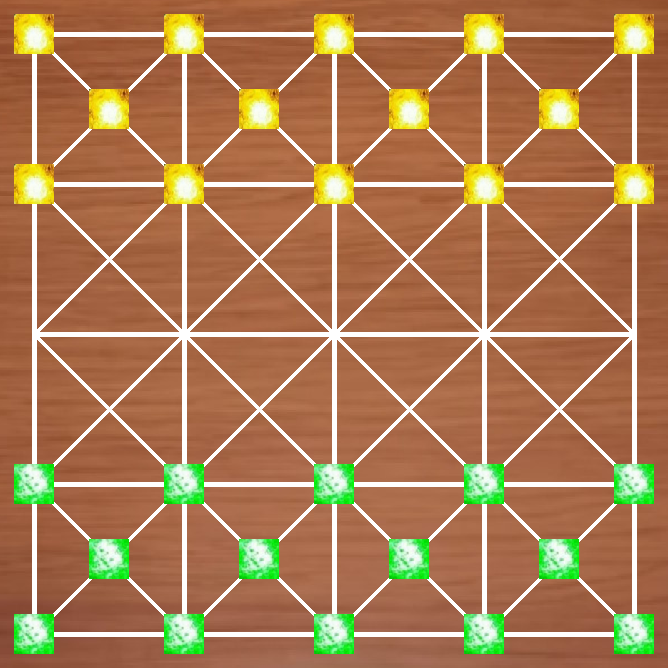
\includegraphics[width=0.5\linewidth]{figures/board_2p.png}
  \caption{The 28 pieces at the starting position (screenshot of the
  software): Yellow and Green, 14 pieces each ($=10$ vertex
  $+\,4$ centre), occupying two rows on opposite sides of the board; the
  three middle rows are empty. Compare
  Equations~\eqref{eq:starty}--\eqref{eq:startg}.}
  \label{fig:start}
\end{figure}

\subsection{Directions---which way pieces move}
\label{ssec:vis_dirs}

\begin{figure}[H]
  \centering
  \begin{subfigure}[b]{0.46\linewidth}\centering
    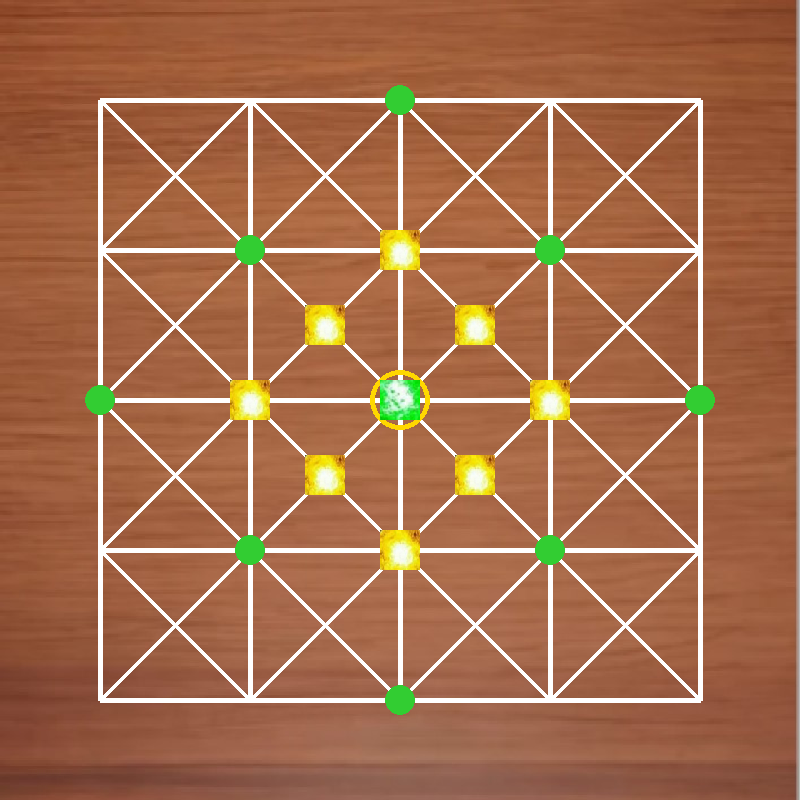
\includegraphics[height=3.4cm]{figures/dir_vertex.png}
    \caption{\textbf{Vertex} piece---8 directions: 4 orthogonal (step 1,
    through an adjacent vertex cell) $+$ 4 diagonal (step $\tfrac12$,
    through a centre cell).}
  \end{subfigure}\hfill
  \begin{subfigure}[b]{0.46\linewidth}\centering
    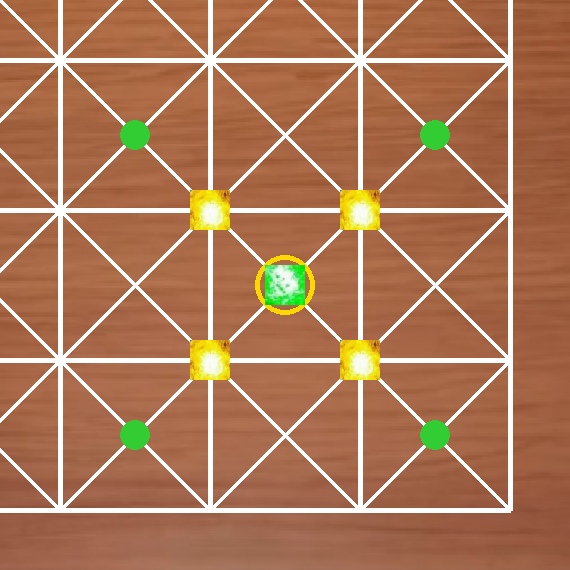
\includegraphics[height=3.4cm]{figures/dir_center.png}
    \caption{\textbf{Centre} piece---only 4 diagonal directions (each step
    through an adjacent vertex cell). Moving orthogonally would fall off
    the centre layer.}
  \end{subfigure}
  \caption{The directions of movement (screenshots of the software; the
  selected piece carries a yellow ring, and the \emph{green dots} are the
  valid landing cells drawn by the software), corresponding to the sets
  $D_{\mathsf V}$ and $D_{\mathsf C}$ in~\eqref{eq:dirs}.}
  \label{fig:dirs}
\end{figure}

\subsection{The jump---the only way to move}
\label{ssec:vis_jump}

A piece moves \emph{only} by jumping: it flies over an adjacent occupied
cell that serves as a \emph{springboard} (of any colour) and lands on the
empty cell immediately beyond it; the springboard piece stays put.
Figure~\ref{fig:jumps} illustrates three kinds of jump.

\begin{figure}[H]
  \centering
  % Example 1: vertex jumps orthogonally
  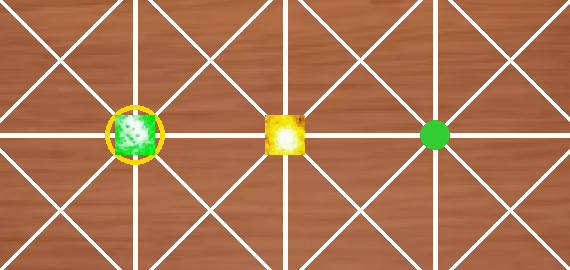
\includegraphics[height=1.9cm]{figures/jump1_before.png}\;$\rightarrow$\;%
  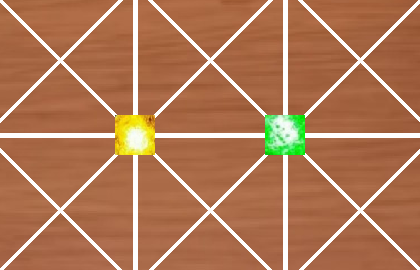
\includegraphics[height=1.9cm]{figures/jump1_after.png}
  \\[0.6em]
  % Example 2: vertex jumps diagonally
  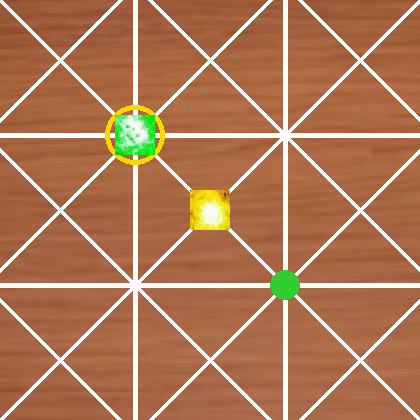
\includegraphics[height=2.3cm]{figures/jump2_before.png}\;$\rightarrow$\;%
  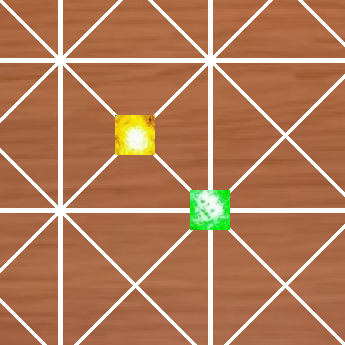
\includegraphics[height=2.3cm]{figures/jump2_after.png}
  \\[0.6em]
  % Example 3: centre jumps diagonally
  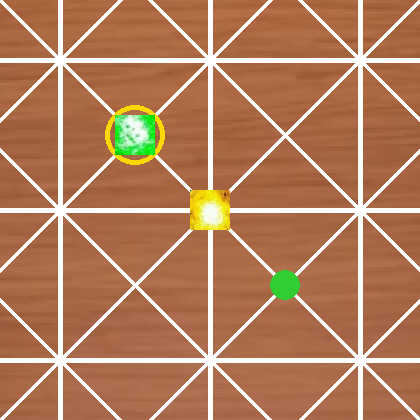
\includegraphics[height=2.3cm]{figures/jump3_before.png}\;$\rightarrow$\;%
  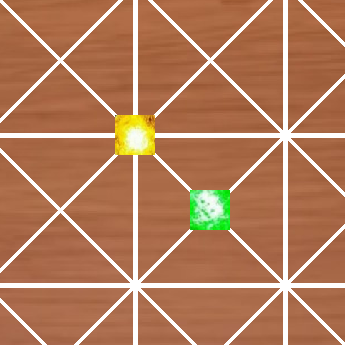
\includegraphics[height=2.3cm]{figures/jump3_after.png}
  \caption{Three jump examples (screenshots of the software, before
  $\rightarrow$ after; yellow ring = selected piece, green dots = valid
  landing cells). \textbf{Top:} a vertex piece jumps orthogonally over the
  springboard $(2,2)$ and lands on $(3,2)$. \textbf{Middle:} a vertex piece
  jumps diagonally using the \emph{centre} cell $(1.5,1.5)$ as springboard
  and lands on the vertex cell $(2,2)$. \textbf{Bottom:} a centre piece
  jumps diagonally using the \emph{vertex} cell $(2,2)$ as springboard and
  lands on the centre cell $(2.5,2.5)$. The springboard always stays in
  place and does not change side.}
  \label{fig:jumps}
\end{figure}

\subsection{Capturing---sandwich and flip}
\label{ssec:vis_capture}

Capture is checked from the landing cell: along each
direction, a run of consecutive opponent pieces immediately followed by one
of your own pieces is sandwiched and changes side.
Figure~\ref{fig:capture} shows a situation with \emph{two} capturing
directions; Table~\ref{tab:capture_rays} lists the details.

\begin{figure}[H]
  \centering
  \begin{subfigure}[b]{0.42\linewidth}\centering
    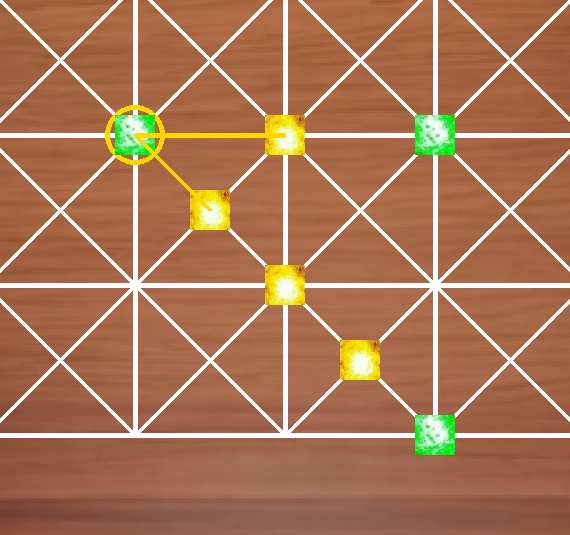
\includegraphics[height=4cm]{figures/capture_before.png}
    \caption{Just landed on $(1,2)$: the game highlights \emph{two}
    capturing rays (yellow).}
  \end{subfigure}\hfill
  \begin{subfigure}[b]{0.42\linewidth}\centering
    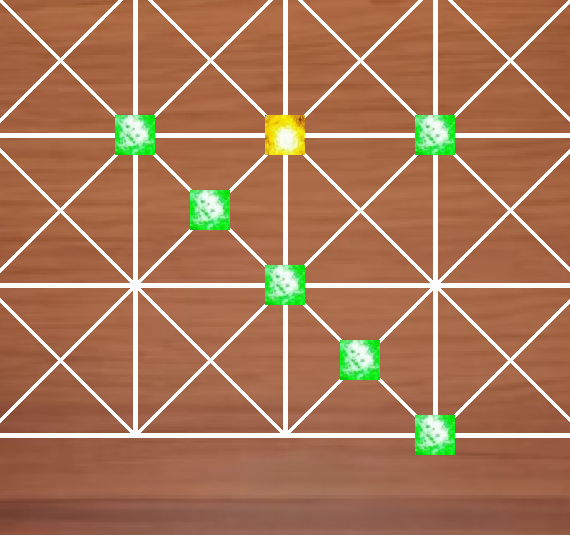
\includegraphics[height=4cm]{figures/capture_after.png}
    \caption{After choosing the diagonal ray and flipping (3 pieces).}
  \end{subfigure}
  \caption{A Green piece has just landed on $(1,2)$ (screenshot of the
  game). There are two capturing directions; the mover chooses
  \emph{one}. Choosing the diagonal ray: the three Yellow pieces
  $(1.5,2.5),(2,3),(2.5,3.5)$ turn Green, while $Y@(2,2)$ on the horizontal
  ray \emph{stays Yellow}---a direction that is not chosen does not flip.}
  \label{fig:capture}
\end{figure}

\begin{table}[H]
  \centering
  \caption{The two capturing directions from landing cell $(1,2)$ in
  Figure~\ref{fig:capture}.}
  \label{tab:capture_rays}
  \setlength{\tabcolsep}{4pt}
  {\small
  \begin{tabular}{lll}
    \toprule
    \textbf{Direction} & \textbf{Ray passes through} & \textbf{Pieces sandwiched} \\
    \midrule
    Horizontal $(1,0)$ & $(2,2){=}\mathrm Y \to (3,2){=}\mathrm G$ & \textbf{1} \\
    Diagonal $(\tfrac12,\tfrac12)$
      & $(1.5,2.5){=}\mathrm y \to (2,3){=}\mathrm Y \to (2.5,3.5){=}\mathrm y \to (3,4){=}\mathrm G$
      & \textbf{3} (2 centre $+$ 1 vertex) \\
    Other directions & broken (hits an empty cell or leaves the board) & 0 \\
    \bottomrule
  \end{tabular}}
\end{table}

\noindent\textbf{Selection rule:} if a sandwich exists you \emph{must}
capture, and you choose exactly \emph{one} direction. Choosing the
direction that captures the most is merely a tactic, not a rule; a player
may capture fewer pieces in order to set a trap.

\subsection{How a move unfolds---three steps}
\label{ssec:vis_move}

\begin{figure}[H]
  \centering
  \begin{subfigure}[b]{0.32\linewidth}\centering
    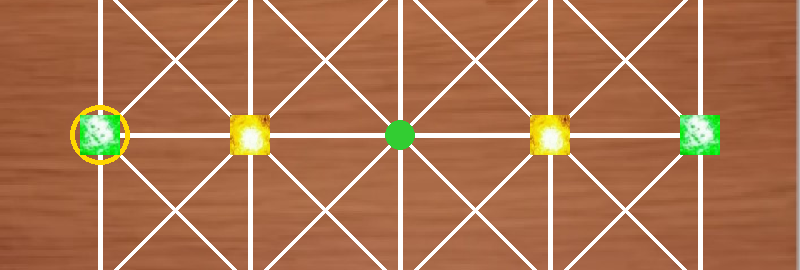
\includegraphics[width=\linewidth]{figures/move_a.png}
    \caption{A. Before the jump.}
  \end{subfigure}\hfill
  \begin{subfigure}[b]{0.32\linewidth}\centering
    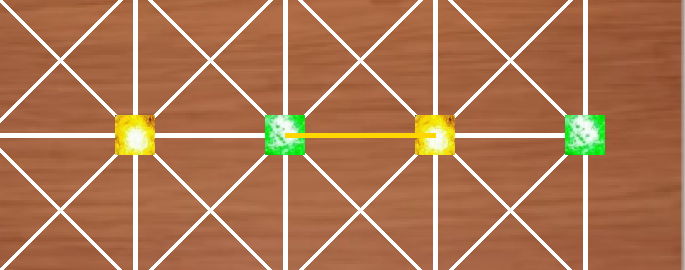
\includegraphics[width=\linewidth]{figures/move_b.png}
    \caption{B. After the jump, before flipping.}
  \end{subfigure}\hfill
  \begin{subfigure}[b]{0.32\linewidth}\centering
    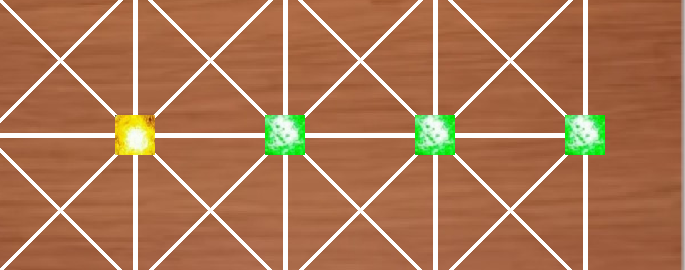
\includegraphics[width=\linewidth]{figures/move_c.png}
    \caption{C. After flipping, turn passes.}
  \end{subfigure}
  \caption{One complete move (screenshots of the software). (A) $G@(0,2)$
  jumps over the springboard $Y@(1,2)$ and lands on $(2,2)$. (B) the
  rightward ray sandwiches $Y@(3,2)$ between the piece that just landed and
  $G@(4,2)$. (C) $Y@(3,2)$ turns Green; the springboard $Y@(1,2)$
  \emph{stays Yellow}; it is now Yellow's turn. The three steps correspond
  to~\eqref{eq:t1}--\eqref{eq:t3}.}
  \label{fig:fullmove}
\end{figure}

\subsection{Turn order}
\label{ssec:turn_order}

Who moves first is agreed among the players; after that the sides move in
turn around the board, one move per turn. The software fixes one clockwise
order: in the 2-player mode Green moves first; in the 3-player mode the
order is Purple $\to$ Yellow $\to$ Green; in the 4-player mode it is
Blue $\to$ Green $\to$ Purple $\to$ Yellow.

\subsection{When the game ends}
\label{ssec:vis_end}

In the 2-player mode, when it is a side's turn and that side has no piece
able to jump, it loses immediately (condition~\eqref{eq:terminal}); the
3--4 player modes are covered in Section~\ref{ssec:elimination}. There are two ways to lose,
shown in Figure~\ref{fig:endgame}.

\begin{figure}[H]
  \centering
  \begin{subfigure}[b]{0.46\linewidth}\centering
    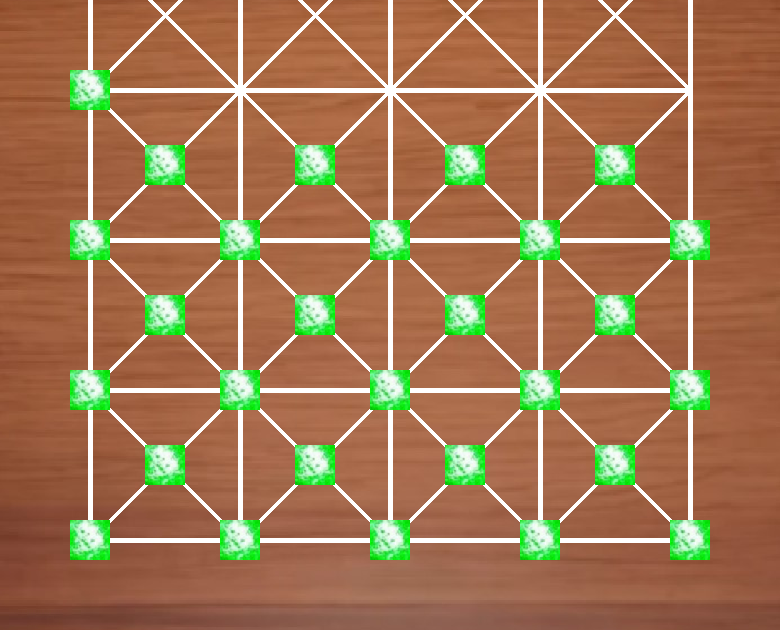
\includegraphics[height=4.2cm]{figures/end_nopieces.png}
    \caption{Out of pieces: all 28 pieces now belong to Green; Yellow has
    nothing left to move.}
  \end{subfigure}\hfill
  \begin{subfigure}[b]{0.46\linewidth}\centering
    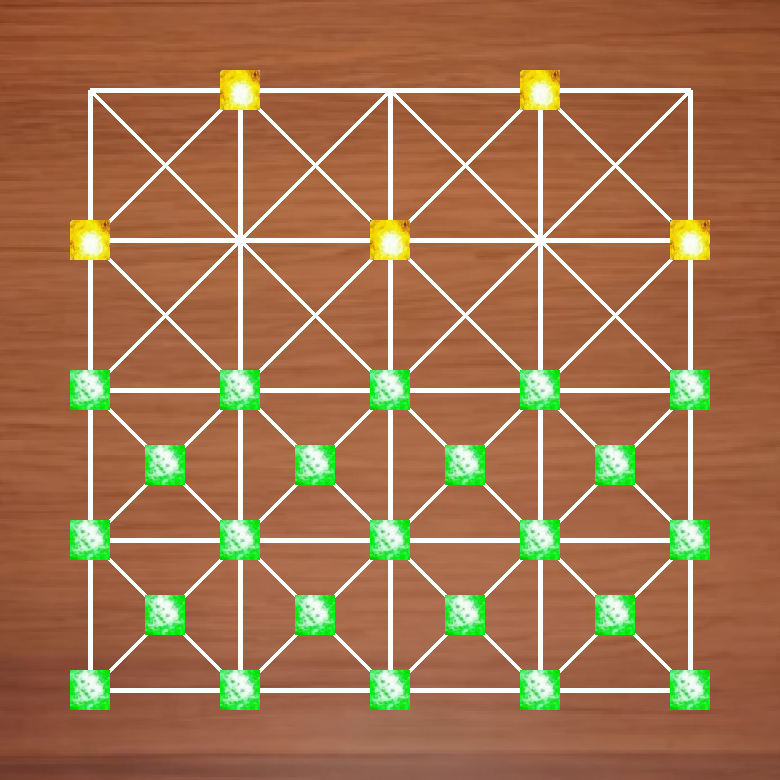
\includegraphics[height=4.2cm]{figures/end_blocked.png}
    \caption{Blockaded: Yellow still has 5 pieces but every landing cell is
    occupied or off the board (a reduced example).}
  \end{subfigure}
  \caption{The two ways to lose. The 2-player mode has no draws. A side that
  temporarily has no move while it is \emph{not} its turn has not yet
  lost---the condition is checked only at the start of its own turn.}
  \label{fig:endgame}
\end{figure}

% !TeX root = ../main.tex
\section{Multiplayer Variants}
\label{sec:variants}

The same core ruleset---movement by jumping, capture by sandwich-flip,
conservation of the total piece count---is kept unchanged across all three
variants; only the board size, the number of pieces per side, and the
number of sides change (Table~\ref{tab:board_size}). The 4-player mode uses
a 7{\texttimes}7 board with eight corner cells removed, forming a
near-octagonal shape balanced for four directions of advance
(Figure~\ref{fig:multiboard}); the 3-player mode uses a 7{\texttimes}6
board with only the two top corners removed.

\begin{figure}[H]
  \centering
  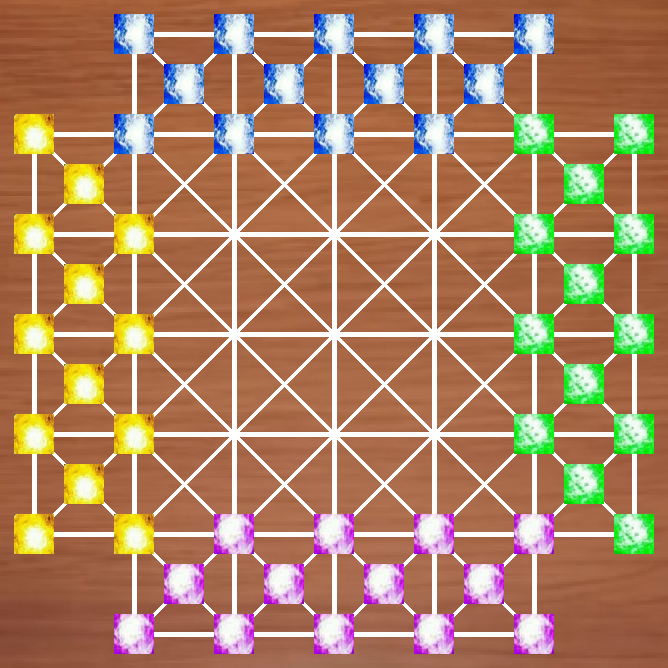
\includegraphics[width=0.52\linewidth]{figures/board_4p.png}
  \caption{Starting position of the 4-player mode (screenshot taken
  directly from the game): a 7{\texttimes}7 board with eight corner cells
  removed, forming a near-octagonal shape balanced for four directions of
  advance; four sides Blue, Green, Purple, and Yellow with 13 pieces each.
  Exact coordinates and starting positions in
  Appendix~\ref{app:multistart}.}
  \label{fig:multiboard}
\end{figure}

\subsection{2-Player Mode}
A 5{\texttimes}5 vertex board. 14 pieces per side (10 vertex + 4 centre).
Colours: Yellow and Green. This is the mode modelled in full in
Appendix~\ref{app:formal} and that uses classic Minimax Alpha-Beta
(Section~\ref{sec:ai}).

\subsection{3-Player Mode}

\begin{figure}[H]
  \centering
  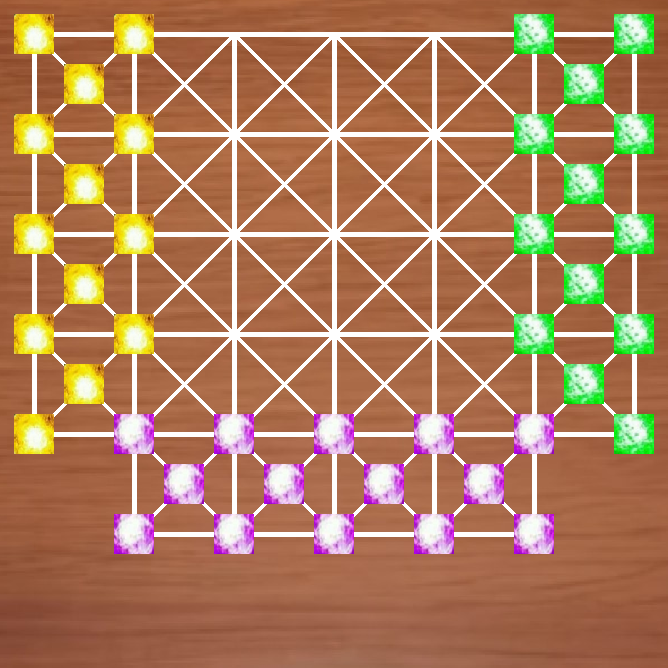
\includegraphics[width=0.52\linewidth]{figures/board_3p.png}
  \caption{Starting position of the 3-player mode (screenshot taken
  directly from the game): a 7{\texttimes}6 board with four cells removed at
  the two top corners; three sides Yellow, Green, and Purple. The
  configuration is \emph{unbalanced}---two sides have 13 pieces and the
  third has 14 (Appendix~\ref{app:multistart}).}
  \label{fig:board3p}
\end{figure}

A 7{\texttimes}6 board with the 4 top corner cells removed. Two sides have
13 pieces and the third side has 14 pieces (exact configuration and the
asymmetry note in Appendix~\ref{app:multistart}). Colours: Yellow, Green,
and Purple. This mode introduces \emph{coalition dynamics}: a player must
consider not only attacking a direct opponent but also avoiding creating an
advantage for a third opponent. Because the score is no longer fully
opposed between two sides, the AI switches to Paranoid Minimax
(Section~\ref{sec:ai})---the pessimistic assumption that the two remaining
opponents coordinate against the player.

\subsection{4-Player Mode}
A 7{\texttimes}7 board with 8 corner cells removed, 13 pieces per side.
Colours: Blue, Green, Purple, and Yellow. Four players create a complex
web of relationships; victory usually comes from holding a neutral position
and then striking decisively once the opponents have worn one another down.

% !TeX root = ../main.tex
\section{Companion AI}
\label{sec:ai}

\subsection{Why an AI Is Needed}

One of the barriers to an abstract board game is the need for an opponent.
A companion AI lets a player practise alone and feel the tactical depth
without having to wait for someone else.

\subsection{Why Not Random-Rollout MCTS}

Monte Carlo Tree Search (MCTS)~\citep{coulom2006efficient,browne2012survey}
is often chosen for multiplayer games because it needs no explicit
evaluation function. The argument below targets \emph{MCTS with plain
random rollouts} (vanilla UCT)---not MCTS in general: the neural-network-%
guided MCTS variant of the AlphaZero kind~\citep{silver2018alphazero}
replaces random rollouts with a learned value function and plays very
strongly even in the Reversi-like class, so it lies outside the scope of
this critique (and is revisited under future work). With plain random
rollouts and a small compute budget, MCTS performs poorly in Tactical
Formation because:
\begin{itemize}
  \item A single move can flip 5--10 pieces at once---the outcome of a
        random game is almost unrelated to the quality of the first move.
  \item The rollout signal is too noisy, and UCT cannot distinguish a good
        move from a bad one.
  \item With a budget of 500--800 simulations, MCTS explores only the first
        1--2 layers, equivalent to greedy 1-ply.
\end{itemize}
This contrasts with Hex, where MCTS rollouts are more effective because the
rollout signal is less noisy~\citep{arneson2010hex}: how well a random
rollout fits depends strongly on its reliability within each class of game.
In the Reversi-like class, an explicit evaluation function based on piece
count and mobility---in the spirit of the learned evaluation functions for
Othello~\citep{buro1999how}---distinguishes move quality better than a
random rollout.

\subsection{Adversarial Search}
\label{ssec:search}

The bot uses \emph{two} separate algorithms depending on the number of
players---both from the Minimax family with Alpha-Beta pruning, but
differing in their evaluation function and in how they handle the endgame.
We write $N_c$ for the number of pieces and $M_c$ for the number of legal
moves (mobility) of side $c$.

\paragraph{2-player mode---Minimax Alpha-Beta.} The two sides are fully
opposed, so the bot uses classic Minimax~\citep{knuth1975alphabeta}
(Algorithm~\ref{alg:minimax}): our side maximises, the opponent minimises,
alternating via the \textsc{max} flag. The evaluation function is designed
to \emph{think like a player}---both wanting to capture pieces and wanting
to squeeze the opponent's space of moves---by normalising both terms to
$[-1,1]$ and then assigning weights $0.7$ and $0.3$ (see the reasoning in
Section~\ref{ssec:pitfalls}):
\begin{equation}
\mathrm{eval}_2(b,c)=0.7\,\frac{N_c-N_{\bar c}}{N_c+N_{\bar c}}
+0.3\,\frac{M_c-M_{\bar c}}{M_c+M_{\bar c}}\ \in[-1,1].
\label{eq:eval}
\end{equation}
When a side is no longer alive, the terminal score carries a fast-win bonus
\begin{equation}
\mathrm{score}^{2}_{\text{term}}=\pm(10000+d)
\label{eq:term2}
\end{equation}
($+$ if the opponent loses, $-$ if we lose; $d$ is the remaining depth).
The terminal value dominates every eval score $\in[-1,1]$, so shrinking the
scale does not make the bot miss a real winning or losing move.

\begin{algorithm}[H]
\caption{Minimax Alpha-Beta (2-player mode)}
\label{alg:minimax}
\begin{algorithmic}[1]
\Function{Minimax}{$s,\ d,\ \alpha,\ \beta,\ \textsc{max},\ \textsc{me},\ \textsc{opp}$}
  \If{$s$ is terminal} \State \Return $\pm(10000+d)$ \Comment{by~\eqref{eq:term2}} \EndIf
  \If{$d=0$} \State \Return $\mathrm{eval}_2(s,\textsc{me})$ \EndIf
  \State $c \gets \textsc{me}$ if \textsc{max}, else $\textsc{opp}$
  \State $\mathit{moves} \gets \mathcal A(c,s)$
  \If{$\mathit{moves}=\varnothing$} \State \Return $\mathrm{eval}_2(s,\textsc{me})$ \EndIf
  \If{\textsc{max}} \Comment{our turn: maximise}
    \State $v \gets -\infty$
    \For{$a \in \mathit{moves}$}
      \State $v \gets \max\bigl(v,\ \textsc{Minimax}(T(s,a),\,d{-}1,\,\alpha,\,\beta,\,\textsf{false},\,\textsc{me},\,\textsc{opp})\bigr)$
      \State $\alpha \gets \max(\alpha, v)$
      \If{$\alpha \ge \beta$} \textbf{break} \Comment{$\beta$ cutoff} \EndIf
    \EndFor
  \Else \Comment{opponent's turn: minimise}
    \State $v \gets +\infty$
    \For{$a \in \mathit{moves}$}
      \State $v \gets \min\bigl(v,\ \textsc{Minimax}(T(s,a),\,d{-}1,\,\alpha,\,\beta,\,\textsf{true},\,\textsc{me},\,\textsc{opp})\bigr)$
      \State $\beta \gets \min(\beta, v)$
      \If{$\alpha \ge \beta$} \textbf{break} \Comment{$\alpha$ cutoff} \EndIf
    \EndFor
  \EndIf
  \State \Return $v$
\EndFunction
\end{algorithmic}
\end{algorithm}

\paragraph{3--4 player mode---Paranoid Minimax.} With $\ge 3$ sides, the
score is no longer fully opposed, so pruning is
harder~\citep{korf1991multiplayer,sturtevant2000pruning}. The bot applies
\textbf{Paranoid Minimax}~\citep{sturtevant2003comparison,sturtevant2008analysis}
(Algorithm~\ref{alg:paranoid}): the side under consideration maximises,
\emph{every other side is treated as a single coalition} that minimises,
reducing the $N$-player problem to a two-sided max--min so that full
Alpha-Beta applies. It keeps the same $0.7/0.3$ weights and the piece-count
term normalised to $[-1,1]$ as in the 2-player mode, but because the
opponents are merged into one coalition, the mobility term is made
\emph{asymmetric}: it measures only the mobility $M_c$ of the side under
consideration (without subtracting the opponents' mobility) and normalises
by the total piece count $T$ to stay within $[0,1)$:
\begin{equation}
\mathrm{eval}_{\text{par}}(b,c)=0.7\,\frac{N_c-N_{\bar c}}{T}
+0.3\,\frac{M_c}{M_c+T},\qquad T=N_c+N_{\bar c},
\label{eq:evalpar}
\end{equation}
where $N_{\bar c}$ is the total piece count of \emph{all} opponents. Unlike
\eqref{eq:eval}, the mobility term here is never negative and is never
compared directly with an opponent; it only rewards a side that still has
many moves (avoiding a blockade)---a pragmatic choice, since the mobility
of a merged coalition does not clearly reflect the threat from each
individual opponent. When only one side remains alive, the terminal score
carries a fast-win bonus
\begin{equation}
\mathrm{score}^{\text{par}}_{\text{term}}=\pm(10000+d),
\label{eq:termpar}
\end{equation}
where $d$ is the remaining depth---encouraging the bot to finish early
rather than prolong the game. A strong alternative is Best Reply
Search~\citep{schadd2011brs}, which often outperforms Paranoid in many
4-player games; we choose Paranoid for its simplicity and because it is good
enough within a real-time compute budget, leaving a comparison with Best
Reply Search to future work.

\begin{algorithm}[H]
\caption{Paranoid Minimax (3--4 player mode)}
\label{alg:paranoid}
\begin{algorithmic}[1]
\Function{Paranoid}{$s,\ d,\ \alpha,\ \beta,\ \textsc{me}$}
  \If{only one side is alive} \State \Return $\pm(10000+d)$ \Comment{by~\eqref{eq:termpar}} \EndIf
  \If{$d=0$} \State \Return $\mathrm{eval}_{\text{par}}(s,\textsc{me})$ \EndIf
  \State $c \gets \textsc{turn}(s)$;\quad $\mathit{moves} \gets \mathcal A(c,s)$
  \If{$\mathit{moves}=\varnothing$} \State \Return \textsc{Paranoid}(drop $c$, pass turn) \Comment{a blockaded side is skipped} \EndIf
  \If{$c = \textsc{me}$} \Comment{maximising layer}
    \State $v \gets -\infty$
    \For{$a \in \mathit{moves}$}
      \State $v \gets \max\bigl(v,\ \textsc{Paranoid}(T(s,a),\,d{-}1,\,\alpha,\,\beta,\,\textsc{me})\bigr)$
      \State $\alpha \gets \max(\alpha, v)$
      \If{$\alpha \ge \beta$} \textbf{break} \EndIf
    \EndFor
  \Else \Comment{all other sides: minimising coalition}
    \State $v \gets +\infty$
    \For{$a \in \mathit{moves}$}
      \State $v \gets \min\bigl(v,\ \textsc{Paranoid}(T(s,a),\,d{-}1,\,\alpha,\,\beta,\,\textsc{me})\bigr)$
      \State $\beta \gets \min(\beta, v)$
      \If{$\alpha \ge \beta$} \textbf{break} \EndIf
    \EndFor
  \EndIf
  \State \Return $v$
\EndFunction
\end{algorithmic}
\end{algorithm}

\begin{table}[H]
  \centering
  \caption{AI parameters by game mode.}
  \label{tab:ai_params}
  \begin{tabular}{lccc}
    \toprule
    \textbf{Mode} & \textbf{Algorithm} & \textbf{Depth}
    & \textbf{Time/move} \\
    \midrule
    2-player & Minimax Alpha-Beta & 6 & $<0.3$\,s \\
    3-player & Paranoid Minimax   & 4 & $<0.5$\,s \\
    4-player & Paranoid Minimax   & 3 & $<0.5$\,s \\
    \bottomrule
  \end{tabular}
\end{table}

The AI runs in a background thread (\texttt{asyncio.run\_in\_executor}) so
that the interface does not freeze while it computes.

\subsection{Pruning effectiveness and move ordering}
\label{ssec:ordering}

The effectiveness of Alpha-Beta pruning depends strongly on the order in
which moves are visited. With branching factor $b$ and depth $d$, the
worst-case number of leaf nodes is $O(b^{d})$---no better than exhaustive
search---but if the best move is always visited first, this drops to
$O(b^{d/2})$, that is, it \emph{doubles} the feasible depth within the same
time budget~\citep{knuth1975alphabeta}. Move ordering is therefore the main
lever for pushing the depths in Table~\ref{tab:ai_params}.

Tactical Formation offers a cheap and natural ordering heuristic: because
each action \emph{foresees} the number of pieces it captures,
$|a|=|F_\delta|$ (Section~\ref{ssec:capture}), the bot visits moves in
\emph{decreasing} order of $|a|$. A move that captures many pieces is
usually strong and so is often the best move, helping pruning trigger
early. When $|a|$ is equal, the bot prefers a move that increases mobility
per Equation~\eqref{eq:eval}. To exploit this ordering fully, both engines
use \emph{make/unmake} of moves instead of copying the state at every node.
The 2-player engine additionally uses a \textbf{transposition table} keyed
by a Zobrist hash---storing the upper/lower/exact Alpha-Beta bounds and
prioritising the recorded best move---to avoid recomputing move sequences
that lead back to the same state; the Paranoid engine does not yet use a
transposition table because keying a state (together with the set of living
sides and the turn pointer) is more complex, left for a later version.
Iterative deepening is not yet implemented and is left for future work.

\subsection{Four design pitfalls and their fixes}
\label{ssec:pitfalls}

When testing the bot, we found four pitfalls that are \emph{not}
implementation bugs but stem from applying a general-purpose algorithm to a
specific ruleset: pieces are conserved (capture $=$ change of side,
Section~\ref{ssec:capture}) and the winning condition is essentially to
\emph{blockade} the opponent rather than to annihilate it. Each pitfall
reflects a wrong implicit assumption in that match. The first three pitfalls
(\#1--\#3) have concrete fixes that apply to both engines (2-player and
Paranoid); the fourth pitfall (\#4) is inherent to any depth-limited search
and is discussed separately at the end.

\paragraph{Pitfall \#1 --- Greedy capture.}
\emph{Cause.} The default move generator, when a move creates several
sandwich directions, keeps only the direction that flips the \emph{most}
pieces ($\arg\max_\delta |F_\delta|$). The bot never considers a smaller
capture, even when the large capture opens up a sandwich counterstrike.
Because pieces are conserved, a move that captures 5 pieces may be flipped
back by the opponent for $\ge 6$ pieces on the very next turn---exactly the
``bait'' that the sandwich rule allows.
\emph{Fix.} Replace the action set $\mathcal A(c,s)$ with the
\emph{expanded} set $\mathcal A^{+}$: each landing cell with $k\ge 2$
sandwich directions generates $k$ separate actions, one per direction. The
bot therefore considers smaller captures too; the search tree itself
(through the eval at deeper layers) decides how much capturing is
beneficial, instead of a fixed greedy rule.

\paragraph{Pitfall \#2 --- Wrong focus in the evaluation function.}
\emph{Cause.} The original evaluation function, $10(N_c-N_{\bar
c})+(M_c-M_{\bar c})$, weighted piece count ten times more heavily than
mobility. But because pieces are conserved, ``capturing everything'' is
nearly impossible; the real path to victory is to squeeze the opponent out
of moves. The bot thus optimised the wrong objective---hoarding pieces
instead of blockading. Moreover, the two terms have different units
(counting pieces versus counting moves), so the $10\!:\!1$ weight ratio
carries no clear meaning.
\emph{Fix.} Normalise both terms to $[-1,1]$ and then assign weights that
reflect a player's intuition: $0.7$ for capturing pieces, $0.3$ for
blocking the opponent's moves (Equations~\eqref{eq:eval}
and~\eqref{eq:evalpar}). A smaller weight for mobility but on the
\emph{same scale} makes it genuinely steer toward a blockade once the
piece-count advantage has saturated.

\paragraph{Pitfall \#3 --- Determinism and move repetition.}
\emph{Cause (two layers).} (i)~\emph{Determinism}: $\arg\max$ always
returns the first best move, so for the same position the bot always plays
identically---finding one winning line means winning identically forever.
(ii)~\emph{Oscillation}: because the eval is a continuous real number, two
moves almost never tie in absolute score, so the ``randomise on a tie''
strategy is useless. Worse, because pieces are conserved, the bot often
pushes a piece out and then pulls it straight back to the same position
($A\!\to\!B\!\to\!A$), forming a loop. Measured over 40 self-play games at
depth~2, each observed for at most its first 200 plies because without the
fix the bots can loop without ever finishing (5040 turns in total), \textbf{37.3\%} of positions were a position
that had \emph{already} appeared in the game---showing how common this
oscillation loop is without intervention. The key point: this pitfall
\emph{cannot} be fixed by intervening in the search---Alpha-Beta, move
ordering, or a transposition table change only the \emph{speed}, not the
\emph{move chosen}---so it must be fixed at the move-selection stage.
\emph{Fix (two mechanisms).}
\begin{itemize}
  \item \textbf{Anti-repetition penalty.} A game keeps a history
        $\mathcal H$ of the Zobrist hashes of \emph{every} position that
        has actually occurred. At the root, a move leading to a position
        $b'$ already in $\mathcal H$ is penalised in proportion to the
        number of repetitions:
        $\mathrm{eval}'(a)=\mathrm{eval}(a)-\lambda\cdot\#\{b'\in\mathcal
        H\}$ with $\lambda=0.5$. Because $\lambda$ is much larger than the
        eval gap between reasonable moves, the bot abandons the
        oscillation loop, yet it still accepts a repetition if that is the
        only move that does not lead to a loss.
  \item \textbf{Randomness within an $\varepsilon$ band.} Instead of an
        ``exact tie'', every move within a band $\varepsilon=0.02$ around
        the best move is treated as equivalent and chosen uniformly at
        random. This creates diversity between games without sacrificing
        quality---moves worse than the best by more than $\varepsilon$ are
        still rejected.
\end{itemize}
After the fix, repeating the same 40-game experiment gives a
position-repetition rate of \textbf{0.0\%} (0 repeated positions over 4069
turns)---the oscillation loop is eliminated entirely. Note that the history
$\mathcal H$ contains only positions that have \emph{already} occurred, so
it does not increase search cost exponentially; it is merely an $O(1)$ hash
lookup at the root.

\paragraph{Pitfall \#4 --- Horizon effect.}
A fourth pitfall in the development log---the \emph{horizon effect}, where a
danger is pushed beyond the search depth---is inherent to any depth-limited
search, not specific to this game. With a $5\times5$ board and depth 6, the
state space is small enough that this effect is negligible, so we leave it
as is rather than adding quiescence search; this is a natural direction for
future work if the board size is increased.

% !TeX root = ../main.tex
\section{Implementation and Software}
\label{sec:impl}

The game is written in Python~3 with the Pygame~2 library. The source is
open at:
\url{https://github.com/quyetops/Tactical-Formation-The-Board-Game}.

The source is organised into independent modules: \texttt{core/} (the rule
engine, board geometry, state), \texttt{ai/} (the Minimax and Paranoid
bots, policy), \texttt{ui/} (Pygame rendering, screens, widgets,
animation), and \texttt{tests/} (rule tests). The technical document
\texttt{docs/formal\_model.md} describes the formal mathematical model and
\texttt{docs/visual\_model.html} provides a visual companion.

\subsection{Mapping the formal model to source code}
\label{ssec:mapping}

The \texttt{core/} module directly implements the definitions in
Appendix~\ref{app:formal}, upholding the principle that \emph{the rule
engine depends on neither the interface nor the AI}:
\begin{itemize}[noitemsep,topsep=2pt]
  \item The state~\eqref{eq:state} is an immutable structure consisting of
        the board configuration $b$ (a cell $\to$ colour map) and the side
        to move.
  \item Move generation implements $\mathrm{Jumps}(x,b)$~\eqref{eq:moves}:
        for each piece of the side to move, it scans the direction set
        $D_{\kappa(x)}$ and filters by the three validity
        conditions~\eqref{eq:jump}.
  \item Sandwich detection implements the ray scan~\eqref{eq:clamp}: from
        the landing cell, along each capturing direction, it gathers the run
        of consecutive opponent pieces until it meets one of its own pieces
        (success), an empty cell, or the board edge (failure).
  \item Applying a move is the transition function
        $T$~\eqref{eq:t1}--\eqref{eq:t3}: jump, flip along the chosen
        direction, pass the turn---purely deterministic, creating no piece
        and deleting no piece (the invariant~\eqref{eq:conservation} is
        checked by an assertion that the total piece count $=28$ in
        \texttt{tests/}).
\end{itemize}
The bots in \texttt{ai/} call only those three operations (generate moves,
apply, evaluate): \texttt{minimax.py} implements
Algorithm~\ref{alg:minimax} for the 2-player mode, and
\texttt{paranoid.py} implements Algorithm~\ref{alg:paranoid} for the 3--4
player mode. Both are fully separated from the rule engine and can be
swapped for another algorithm without touching \texttt{core/}.

\begin{lstlisting}[language=bash, caption={Installing and running the game.}]
python -m venv .venv
source .venv/bin/activate   # Linux / macOS
pip install pygame
python main.py
\end{lstlisting}

The web version runs through \texttt{pygbag}~\citep{pygbag}:
\begin{lstlisting}[language=bash, caption={Running in the browser.}]
pip install pygbag
pygbag main.py
# Open the browser at http://localhost:8000
\end{lstlisting}

% !TeX root = ../main.tex
% ─────────────────────────────────────────────────────────────
%  EMPIRICAL EVALUATION — real numbers from experiments/run_eval.py
%  Source CSVs: experiments/results/{branching,gamelength_random,firstmove,
%               tournament,elo,timing,antirep}.csv  (see results/NOTES.md)
% ─────────────────────────────────────────────────────────────
\section{Empirical Evaluation}
\label{sec:eval}

This section quantifies three aspects of Cờ Trận: (i) the
breadth of the game tree via the \emph{branching factor} and game length, (ii) the relative
strength of the AI via a bot-vs-bot tournament, and (iii) real-time
performance. The goal is to confirm that the move space is \emph{broad and
non-degenerate} (branching factor), and that search depth \emph{actually
translates into playing strength} (greater depth beats lesser depth
consistently). Separation by depth is a sign, though not full proof,
that decisions in Cờ Trận have lasting consequences.

\subsection{Experimental Setup}
\label{sec:eval_setup}

All experiments run on an AMD Ryzen~7 6800H CPU (16 threads, 7.4\,GB RAM),
Python~3.12 on Linux (WSL2); the AI search runs single-threaded. The
measurement code lives in \texttt{experiments/} in the open-source
repository, with every random seed fixed for reproducibility. Because Cờ
Trận has no move limit and no draw rule (Section~\ref{sec:provenance}),
every game in the experiments of this section is played until one side
wins. The measurement code sets only a safety cap of $10^5$ plies against an
endless loop, and no game reached it. Each pairing
consists of 50 games; to balance the first-mover advantage, the two bots
alternate going first (each leads 25 games). The bots use the same
evaluation function from Equation~\eqref{eq:eval}, differing only in search
depth. Because each move at depth~6 costs several seconds on the pure Python
interpreter (see Section~\ref{sec:eval_timing}), the number of games is set
at 50 per pairing---enough for the depth-induced difference to show clearly
while staying within the compute budget.

\subsection{Branching Factor and State Space}
\label{sec:eval_branching}

Table~\ref{tab:branching} reports the average number of legal moves
(branching factor) by game phase (early/mid/late by thirds of game length).
It is measured over 60 complete games per mode, that is, about 20,000 sample
positions in the 2-player mode, 94,000 in the 3-player mode and 215,000 in
the 4-player mode. The sample
positions are generated by \emph{legal random play} (each turn picks a move
uniformly from the set of legal moves); the figures therefore reflect the
distribution of positions under random play, which may differ from the
distribution of positions that arise between two strong bots, but they give
an unbiased estimate of the breadth of the game tree. Under random play, a
game lasts a median of 304 plies in the 2-player mode, 1,326 plies in the
3-player mode and 3,259 plies in the 4-player mode. This does not measure
games between real people, but it is consistent with the recollection that
a four-player game used to last three to four hours
(Section~\ref{sec:provenance}).

\begin{table}[H]
  \centering
  \caption{Average branching factor (number of legal moves) by game phase
  and mode. Counting the choice of sandwich direction, the full number of
  \emph{actions} is only marginally higher (2-player $\approx 11.6$;
  3-player $\approx 18.9$; 4-player $\approx 21.1$). 60 random games per mode,
  each played to the end.}
  \label{tab:branching}
  \begin{tabular}{lccc}
    \toprule
    \textbf{Phase} & \textbf{2-player} & \textbf{3-player} & \textbf{4-player} \\
    \midrule
    Early game & 11.3 & 15.7 & 15.8 \\
    Mid game   & 11.1 & 19.0 & 21.7 \\
    Late game  & 11.1 & 20.5 & 22.8 \\
    \midrule
    \textbf{Game average} & 11.1 & 18.4 & 20.1 \\
    \bottomrule
  \end{tabular}
\end{table}

\noindent In the 2-player mode the average branching factor is $\approx 11$
and almost constant across game phases. This is a consequence of the
piece-conservation invariant: the piece count, and hence the number of
potential jumps, does not dwindle as in games with piece removal. In the 3-
and 4-player modes the branching factor \emph{grows} during the game, from
about 16 in the early game to 20--23 in the late game, and the 4-player mode
is the highest. We have not analysed the cause of this trend. All three
modes branch more than Reversi, which has about 10 moves per
turn~\citep{allis1994searching}. These values lie far below the analytic
upper bound $|\mathcal A(s)|\le 1408$ (Appendix~\ref{app:formal}),
confirming that the jump constraint tightens the actual move space;
positioning a game's complexity relative to solved games is standard
evaluation practice~\citep{herik2002games}, and Appendix~\ref{app:formal}
bounds the 2-player state space at about $3.7\times10^{17}$~\eqref{eq:statespace}. It must be stressed: the
branching factor measures the \emph{breadth} of the game tree, not directly
the \emph{depth} of tactics; it only shows that the move space is rich
enough and does not degenerate toward the endgame. The evidence for tactical
depth---that decisions truly matter---comes from the tournament in
Section~\ref{sec:eval_tournament}.

\subsection{Bot-vs-Bot Tournament}
\label{sec:eval_tournament}

To test whether the AI exploits search depth, we have bots of different
depths play adversarially (Table~\ref{tab:tournament}).

\begin{table}[H]
  \centering
  \caption{Bot-vs-bot results, 2-player mode (A is the deeper side; 50
  games per pairing, alternating first move 25/25). The 95\% confidence
  interval of the win-rate is computed by the Wilson method. The rules have
  no draws; every game in all three pairings ended with a winner.}
  \label{tab:tournament}
  \setlength{\tabcolsep}{4.5pt}
  \begin{tabular}{lccccc}
    \toprule
    \textbf{Pairing (depth)} & \textbf{Games} & \textbf{A wins}
      & \textbf{B wins} & \textbf{Win-rate A}
      & \textbf{95\% CI} \\
    \midrule
    d=6 vs d=2 & 50 & 50 & 0 & 100.0\,\% & [92.9,\,100.0] \\
    d=6 vs d=4 & 50 & 43 & 7 & 86.0\,\% & [73.8,\,93.0] \\
    d=4 vs d=2 & 50 & 45 & 5 & 90.0\,\% & [78.6,\,95.7] \\
    \bottomrule
  \end{tabular}
\end{table}

\paragraph{Elo Estimation.}
From the win-rate $p$ of the stronger side, the Elo difference is estimated
as $\Delta\mathrm{Elo} = -400\,\log_{10}(1/p - 1)$. Taking the depth-2 bot
as the 1000-Elo anchor, the d=4 vs d=2 pairing (90.0\%) gives
$\Delta\mathrm{Elo}\approx{+}382$, so depth~4 is $\approx 1382$ Elo, and the
d=6 vs d=4 pairing (86.0\%) gives ${+}315$. Chained together, depth~6 is
$\approx 1697$ Elo, about ${+}697$ above depth~2.\footnote{The d=6 vs d=2 pairing is a clean sweep (100\%),
which makes the logistic formula diverge ($p\to1$ sends
$\Delta\mathrm{Elo}\to\infty$), so it gives only a \emph{lower bound} rather
than a finite Elo value; we therefore estimate the depth-6 Elo via the
d=2\,$\to$\,d=4\,$\to$\,d=6 chain, which is more reliable.}

\paragraph{First-Mover Advantage.}
To probe a basic balance aspect of the 2-player mode, we have two bots of
\emph{equal depth} ($d{=}2$) self-play 100 games (fixed seed). The result is
notable: the \emph{second} mover (Yellow) wins 61 games and the \emph{first}
mover (Green) wins 39. Every game ended with a winner; the longest lasted
313 plies. The first mover's win rate is only $39.0\%$ (95\% Wilson
confidence interval $[30.0,\,48.8]$, lying entirely below $50\%$). Thus, for depth-2 bots,
\emph{moving second is advantageous} in a statistically significant way.
One hypothesis is that in a sandwich-flip game the second mover can
counterstrike after the opponent has revealed its position; we have not
tested this hypothesis. This
is an observation at \emph{one} fixed depth; the advantage may change with
depth and is a next step for the balance study.

\subsection{Real-Time Performance}
\label{sec:eval_timing}

Table~\ref{tab:timing} reports the per-move think time measured in
practice, for exactly the configurations in Table~\ref{tab:ai_params}.

\begin{table}[H]
  \centering
  \caption{Think time per move (seconds), measured over every move of 3
  complete self-play games per configuration (2-player: 919 moves;
  3-player: 2,029 moves; 4-player: 1,179 moves). The three configurations ran
  in parallel, one process per core; each search is still single-threaded,
  as in the game.}
  \label{tab:timing}
  \begin{tabular}{lccc}
    \toprule
    \textbf{Mode (depth)} & \textbf{Median} & \textbf{95th percentile}
      & \textbf{Max} \\
    \midrule
    2-player (d=6) & 3.07 & 5.80 & 9.51 \\
    3-player (d=4) & 1.11 & 2.35 & 4.47 \\
    4-player (d=3) & 0.17 & 0.57 & 1.40 \\
    \bottomrule
  \end{tabular}
\end{table}

\subsection{Discussion of Results}
\label{sec:eval_discussion}

Three observations emerge from the measurements above.

\textbf{(1) The move space is broad and non-degenerate.} A branching factor
of $\approx 11$ in the 2-player mode and $\approx 18$--$20$ in the 3- and
4-player modes (Table~\ref{tab:branching}) shows that each turn offers many
choices. In no mode does the branching shrink toward the end of the game: it
is stable in the 2-player mode and even grows in the 3- and 4-player modes,
unlike games with piece removal, where the branching dwindles toward the
endgame. The game therefore does not degenerate into a simple endgame.
Branching alone does not prove tactical depth; it establishes a necessary
condition (a non-trivial space), while the sufficient evidence comes from
observation~(2).

\textbf{(2) Search depth translates into playing strength (the evidence for
tactical depth).} The win-rate ranks monotonically with depth---d=6 beats
d=2 absolutely (100\%), d=4 beats d=2 (90\%), and d=6 beats d=4 (86\%)
(Table~\ref{tab:tournament})---every game ended with a winner, and all 95\%
confidence intervals lie clearly above $50\%$. That seeing farther brings a
systematic advantage indicates that decisions in Cờ Trận \emph{have
long-term consequences}---a sign of tactical depth---and that the evaluation
function combined with Minimax search is ``meaningful'', not random noise.
The Elo estimate above quantifies the gap: every two depth
levels correspond to $\approx 300$--$380$ Elo. Note that this is an
\emph{intrinsic} scale (relatively anchored among bots of the same engine),
not an Elo anchored to human players or an external opponent; it shows that
\emph{relative} strength grows with depth, not the absolute quality of the
AI.

\textbf{(3) Real-time performance.} The 4-player mode has a median of
$0.17$\,s per move, comfortable for interaction. The 3-player mode at
depth~4 takes a median of $1.11$\,s, at most $4.5$\,s. The 2-player mode at
depth~6 takes a median of $3.07$\,s and at most $9.5$\,s per move on the
single-threaded pure Python interpreter---beyond the threshold for instant
feedback. This is a strength--speed trade-off; it could be reduced by
adaptive depth reduction, time-limited search, or a compiled
implementation.

In summary, the experiments confirm both goals set at the start of the
section: the game \emph{does} have measurable tactical depth and the AI
\emph{plays reasonably}, with a clear time cost for the deepest search
configuration.

% !TeX root = ../main.tex
\section{Limitations}
\label{sec:limitations}

The main limitation lies in the source material. The rules of Cờ Trận were
recorded from the recollection of \emph{one} person, the author, many years
after they stopped playing (Section~\ref{sec:provenance}). We have not found
a second person to cross-check them, nor any written document. The record
may therefore differ from how the game was played at other times, by other
groups of children in the village, or in neighbouring villages, and errors of
memory cannot be ruled out. We have no information about the longer history
of the game: when it arose, who devised it, or whether it is related to any
other game.

The software does not yet have an online mode for remote multiplayer play.
The AI's evaluation function uses only two features (piece count and
mobility); deeper strategic factors such as centre control, multi-direction
threats, or positional value are not modelled.

The formal mathematical model in Appendix~\ref{app:formal} is complete only
for the 2-player mode. The extension to 3 and 4 players is specified only at
the configuration level (board size, starting positions---%
Appendix~\ref{app:multistart}) and has not been analysed theoretically,
especially the balance properties of multiplayer games. Notably, the
starting configuration of the 3-player mode is \emph{unbalanced}: two sides
have 13 pieces while the third has 14. We record this configuration exactly
as in the folk game and do \emph{not} alter it, since changing the rules
would falsify the record. Any more balanced version would have to be
presented clearly as a new variant; automated balance measurement and design
methods~\citep{hommarks2007balanced} offer one way to explore this.

The bot-vs-bot tournament in Section~\ref{sec:eval} has so far only compared
search depths in the 2-player mode. The first-mover advantage measurement
(Section~\ref{sec:eval_tournament}) is also only in the 2-player mode and at
one fixed depth ($d{=}2$, where the second mover appears to have an
advantage); there is no quantitative study yet of the balance among colours
in the 3- and 4-player modes---the questions of whether moving first or
second confers a systematic advantage at other depths, and whether an
implicit coalition strategy is stable, remain open.

As for the terminal condition, Cờ Trận has \emph{no} move limit and no
repetition-based draw rule, in any mode. In theory a game could go on forever
without any side being blockaded. This is a property of the folk game itself:
in real play, a four-player game could last three to four hours
(Section~\ref{sec:provenance}). The software keeps it that way and sets no
move limit. The AI's anti-repetition mechanism (Section~\ref{ssec:pitfalls})
makes endless repetition rare when the machine plays, but the rules do not
rule it out.

% !TeX root = ../main.tex
\section{Conclusion}
\label{sec:conclusion}

This paper has recorded Cờ Trận, a folk board game of the children of Đồng
Bùa hamlet (Tam Quan, Tam Đảo, Vĩnh Phúc), which to our knowledge had never
been written down. The rules for all three modes, for 2, 3 and 4 players,
were recorded from the author's recollection and specified completely and
consistently. Cờ Trận belongs to the family of games that capture by
conversion, together with Reversi, Cờ gánh and Ming Mang. What sets it apart
is the combination of Halma-style movement by jumps only, straight-line
sandwich capture in a single chosen direction, and a two-layer
vertex--centre board. The formal mathematical model for the 2-player mode
clarifies the 28-Piece Conservation Law, a formal statement of the principle
``capture = change of side, never removal''.

The companion AI, based on Minimax search with Alpha-Beta pruning (the
Paranoid variant for the multiplayer modes), plays reasonably within an
interactive time budget and lets a player practise alone when no opponent is
available; the bot-vs-bot tournament confirms that deeper search wins
consistently. The open-source software is a second form of preservation
alongside the written record: anyone can play Cờ Trận again, even if nobody
left in the village remembers the rules.

\paragraph{Future directions.}
\begin{enumerate}[label=(\roman*)]
  \item Find other people who played Cờ Trận in Đồng Bùa and neighbouring
        villages, to cross-check the rules and record any local variants.
  \item Attempt to solve the 2-player mode, whose state space is at most
        about $3.7\times10^{17}$~\eqref{eq:statespace}.
  \item Extend the formal mathematical model to the 3- and 4-player modes,
        analysing the existence of equilibrium strategies and coalition
        dynamics.
  \item Quantitatively analyse game balance through bot-vs-bot simulation
        over hundreds of games, estimating the first-mover advantage if any.
  \item Compare Paranoid Minimax experimentally with Best-Reply
        Search~\citep{schadd2011brs}.
  \item Improve the AI's evaluation function with more complex strategic
        features, or learn the evaluation function through self-play in the
        AlphaZero direction~\citep{silver2018alphazero}.
  \item Develop an online mode to support remote multiplayer play.
  \item Describe Cờ Trận in the general game system
        Ludii~\citep{piette2020ludii}, to archive it alongside other
        traditional games and allow automatic play and comparison.
\end{enumerate}


% ── Appendices ───────────────────────────────────────────────────
\appendix
% !TeX root = ../main.tex
\section{Formal Mathematical Model (2-Player Mode)}
\label{app:formal}

This appendix specifies Tactical Formation mathematically,
\emph{independently of any software implementation}, complementing the
presentation through images in Section~\ref{sec:rules} (which is
enough to grasp the rules). The focus is on the core of the game: which
\textbf{direction} a piece moves in and how it \textbf{captures}. The model
rests on three pillars---\textbf{state}, \textbf{action},
\textbf{reward}---and one principle throughout: \emph{the board always has
exactly 28 pieces; capture is a change of side, never removal}. The
extension to the 3--4 player modes is given in Section~\ref{sec:variants}.

\subsection{The board and the 28 pieces}
\label{ssec:board}

The 2-player board consists of 41 cells on two layers:
\begin{align}
\mathcal{B}_{\mathsf V}
  &= \{(i,j)\in\mathbb Z^2 : 0\le i,j\le 4\}
  && \text{(25 vertex cells)}, \label{eq:vert}\\
\mathcal{B}_{\mathsf C}
  &= \{(i{+}\tfrac12,\,j{+}\tfrac12) : 0\le i,j\le 3\}
  && \text{(16 centre cells)}, \label{eq:cent}\\
\mathcal{B}
  &= \mathcal{B}_{\mathsf V}\sqcup\mathcal{B}_{\mathsf C},
  && |\mathcal{B}|=41. \label{eq:board}
\end{align}
Each centre cell lies exactly in the middle of the four surrounding vertex
cells. The type function $\kappa(x)\in\{\mathsf V,\mathsf C\}$ tells whether
cell $x$ is a vertex or a centre. The two sides are $\mathcal C=\{\mathrm
Y,\mathrm G\}$ (Yellow, Green); the opponent of $c$ is written $\bar c$; an
empty cell is denoted $\varnothing$. By convention, Green moves first
(Section~\ref{ssec:turn_order}).

The game has exactly \textbf{28 pieces}; each side starts with 14 pieces
($=10$ vertex pieces $+\,4$ centre pieces). Each piece $p$ carries three
attributes:
\begin{itemize}[noitemsep,topsep=2pt]
  \item \textbf{type} $\kappa(p)\in\{\mathsf V,\mathsf C\}$---\emph{invariant
        for the whole game}: a vertex piece always stays on vertex cells, a
        centre piece on centre cells;
  \item \textbf{position} $x_p$---changes when the piece jumps;
  \item \textbf{side} $c_p\in\{\mathrm Y,\mathrm G\}$---changes when the
        piece is captured.
\end{itemize}

\begin{quote}
\textbf{The 28-piece conservation invariant.} No piece is ever added to or
removed from the board; capture is a \emph{change of side} of an existing
piece. Therefore, at every state
\begin{equation}
N_{\mathrm Y}(s)+N_{\mathrm G}(s)=28,
\label{eq:conservation}
\end{equation}
where $N_c(s)$ is the number of pieces of side $c$.
\end{quote}

We should be clear about the status of this claim: it is an \emph{invariant
that follows directly from the definition}---because capture is defined as
\emph{flipping the colour} of an existing piece (no addition, no removal),
the total piece count obviously does not change---rather than a deep theorem
needing an elaborate proof. Its value lies in its \emph{consequence for
play}: the game never degenerates into a sparse endgame, and all 28 pieces
always stay in play.

The invariant~\eqref{eq:conservation} distinguishes Tactical Formation from
both Checkers (capture $=$ removal) and Reversi (the piece count grows with
each placement), and places it in the same group as Shoulder-Pole Chess and Ming Mang,
two games that also conserve the total number of pieces
(Section~\ref{sec:related}). The starting position (state $0$) consists of two
symmetric blocks of pieces:
\begin{align}
P^{\mathrm Y}_0 &= \{(i,0)\}_{i=0}^{4}\cup\{(i{+}\tfrac12,\tfrac12)\}_{i=0}^{3}\cup\{(i,1)\}_{i=0}^{4},
\label{eq:starty}\\
P^{\mathrm G}_0 &= \{(i,4)\}_{i=0}^{4}\cup\{(i{+}\tfrac12,\tfrac72)\}_{i=0}^{3}\cup\{(i,3)\}_{i=0}^{4}.
\label{eq:startg}
\end{align}

\subsection{State}
\label{ssec:state}

The game state is the pair
\begin{equation}
\boxed{\;s=(b,\mathrm{turn}),\qquad
b:\mathcal B\to\{\mathrm Y,\mathrm G,\varnothing\},\qquad
\mathrm{turn}\in\{\mathrm Y,\mathrm G\}.\;}
\label{eq:state}
\end{equation}
$b$ is the \emph{board configuration} (which cell holds which colour), and
$\mathrm{turn}$ is the side to move. The position and side of all 28
pieces together with the side to move determine the entire state; the game is one of
\emph{perfect information}, with no hidden information. The starting state is
$s_0=(b_0,\mathrm G)$ (by convention Green moves first; in real play the
first mover is agreed among the players) with $b_0$ placed per
\eqref{eq:starty}--\eqref{eq:startg}. The piece-count function $N_c(s)$
satisfies $N_{\mathrm Y}(s_0)=N_{\mathrm G}(s_0)=14$ and the
invariant~\eqref{eq:conservation}.

\subsection{Directions and the jump}
\label{ssec:action}

The set of movement directions depends on the piece type:
\begin{equation}
D_{\mathsf V} = \underbrace{\{(\pm1,0),(0,\pm1)\}}_{\text{4 orthogonal, step }1}
  \cup \underbrace{\{(\pm\tfrac12,\pm\tfrac12)\}}_{\text{4 diagonal, step }\frac12},
\qquad
D_{\mathsf C} = \{(\pm\tfrac12,\pm\tfrac12)\}.
\label{eq:dirs}
\end{equation}
A vertex piece has 8 directions; a centre piece has only 4 diagonal
directions (moving orthogonally by one cell would fall off the centre
layer). A piece at cell $x$ moves along $d\in D_{\kappa(x)}$ by jumping
\emph{over} the adjacent cell $x+d$ and \emph{landing} on $x+2d$. A jump is
valid if and only if
\begin{equation}
\underbrace{x{+}d,\ x{+}2d\in\mathcal B}_{\text{stays on the board}},
\qquad
\underbrace{b(x{+}d)\neq\varnothing}_{\text{springboard occupied (any colour)}},
\qquad
\underbrace{b(x{+}2d)=\varnothing}_{\text{landing cell empty}}.
\label{eq:jump}
\end{equation}
Because $2d$ is an integer vector, the landing cell is automatically of the
same type as $x$ (vertex to vertex, centre to centre). \textbf{The
springboard piece stays put}---it does not move and does not change side.
The set of valid landing cells and the set of moves are
\begin{equation}
\begin{aligned}
\mathrm{Jumps}(x,b)&=\{x{+}2d : d\in D_{\kappa(x)},\ \eqref{eq:jump}\ \text{holds}\},\\
\mathcal A_{\mathrm{move}}(s)&=\{(x,x') : b(x)=\mathrm{turn},\ x'\in\mathrm{Jumps}(x,b)\}.
\end{aligned}
\label{eq:moves}
\end{equation}
The springboard for a vertex piece moving diagonally is a \emph{centre}
cell; the springboard for a centre piece is a \emph{vertex} cell---the two
layers interlock through the diagonals (see the illustration in
Figure~\ref{fig:jumps}).

\subsection{Capturing---the core of the game}
\label{ssec:capture}

In short: from the
landing cell, along each direction, if you see a run of consecutive opponent
pieces immediately followed by one of your own pieces, then the whole run is
\emph{sandwiched} and \emph{changes side} to yours. Capturing uses the same
direction set as movement: a vertex piece considers
$\Delta_{\mathsf V}=D_{\mathsf V}$ (8 directions), a centre piece considers
$\Delta_{\mathsf C}=D_{\mathsf C}$ (4 diagonal directions). The \emph{ray} in
direction $\delta$ from the landing cell $x'$ is the sequence of cells
$x'+\delta,\ x'+2\delta,\ x'+3\delta,\dots$; an orthogonal ray passes only
through vertex cells, while a diagonal ray alternates
centre--vertex--centre, so a diagonal sandwich can capture both vertex and
centre pieces.

Let $b'$ be the board right after the jump (jumped, not yet flipped) and
$c=\mathrm{turn}$. Direction $\delta$ \textbf{captures} when there exists an
integer $m\ge 1$ such that
\begin{equation}
\underbrace{b'(x'+k\delta)=\bar c,\quad k=1,\dots,m}_{m\ \text{consecutive opponent pieces}},
\qquad
\underbrace{b'(x'+(m{+}1)\delta)=c}_{\text{a friendly piece right after the run}}.
\label{eq:clamp}
\end{equation}
Then the flip set of direction $\delta$ is $F_\delta=\{x'+k\delta : 1\le
k\le m\}$. Direction $\delta$ does \emph{not} capture (by convention
$F_\delta=\varnothing$) if the ray---before reaching one of your own
pieces---hits an empty cell, leaves the board, or immediately meets one of
your own pieces (with no opponent piece in between). The set of capturing
directions of move $(x,x')$ is $\Delta(s,x,x')=\{\delta :
F_\delta\neq\varnothing\}$.

\paragraph{The full action.} An action is the triple
\begin{equation}
\boxed{\;a=(x,\ x',\ \delta)\;}
\qquad
\delta\in
\begin{cases}
\Delta(s,x,x') & \text{if a capturing direction exists},\\
\{\varnothing\} & \text{otherwise (no flip)},
\end{cases}
\label{eq:action}
\end{equation}
with $(x,x')\in\mathcal A_{\mathrm{move}}(s)$. \textbf{Rule:} if a sandwich
exists the player \emph{must capture}, and chooses \emph{exactly one
direction}---the other capturing directions do not flip. Every $F_\delta$
can be computed directly from the board-after-the-jump, so the mover always
foresees how many pieces each capturing choice takes.
\paragraph{Example.} \emph{Notation convention in this example:} uppercase
$\mathrm Y,\mathrm G$ denotes \emph{vertex} pieces, lowercase
$\mathrm y,\mathrm g$ denotes \emph{centre} pieces (of the same
Yellow/Green colour); this is merely shorthand to make each piece's layer
visible---the board function $b$ in~\eqref{eq:state} still returns only a
colour, while the layer is the attribute $\kappa(x)$ of the cell. A Green
piece ($c=\mathrm G$) has just landed on $x'=(1,2)$ with the surrounding
configuration: $b'(2,2)=\mathrm Y$, $b'(3,2)=\mathrm G$ on the horizontal
ray; and $b'(1.5,2.5)=\mathrm y$, $b'(2,3)=\mathrm Y$,
$b'(2.5,3.5)=\mathrm y$, $b'(3,4)=\mathrm G$ on the diagonal ray. The two
capturing directions:
\begin{align}
\delta_1=(1,0):\quad & F_{\delta_1}=\{(2,2)\}, && |{\cdot}|=1, \label{eq:ex1}\\
\delta_2=(\tfrac12,\tfrac12):\quad & F_{\delta_2}=\{(1.5,2.5),(2,3),(2.5,3.5)\}, && |{\cdot}|=3. \label{eq:ex2}
\end{align}
The diagonal ray~\eqref{eq:ex2} captures both centre and vertex pieces (2
centre $+$ 1 vertex), illustrating how a diagonal ray alternates between the
two layers. The mover chooses exactly one direction; choosing $\delta_2$,
the three Yellow pieces on the diagonal ray turn Green, while $Y@(2,2)$ on
the horizontal ray \emph{stays Yellow}. This situation is shown visually in
Figure~\ref{fig:capture} and Table~\ref{tab:capture_rays}.

\subsection{Reward}
\label{ssec:reward}

The size of an action is the number of pieces it captures, $|a|:=|F_\delta|$
(equal to $0$ if $\delta=\varnothing$). The per-step reward is zero-sum:
\begin{equation}
\boxed{\;r_c(s,a)=+|a|,\qquad r_{\bar c}(s,a)=-|a|\;}
\qquad (c=\mathrm{turn}).
\label{eq:reward}
\end{equation}
Four direct consequences of \emph{capture $=$
change of side}:
\begin{enumerate}[label=(\arabic*),noitemsep,topsep=2pt]
  \item \textbf{Zero-sum per step:} $r_{\mathrm Y}(s,a)+r_{\mathrm G}(s,a)=0$.
  \item \textbf{Capturing $k$ pieces swings the piece-count difference by
        $2k$:} us $+k$, opponent $-k$ at once.
  \item \textbf{The total is always 28:} the invariant~\eqref{eq:conservation}
        at every state.
  \item \textbf{The scoreboard is the board itself:} along a game
        $s_0,a_0,s_1,\dots,s_t$,
        \begin{equation}
        N_c(s_t)=14+\sum_{k=0}^{t-1} r_c(s_k,a_k);
        \label{eq:scoreboard}
        \end{equation}
        counting each side's pieces at any moment reads off that side's
        cumulative reward.
\end{enumerate}
When the game ends, the winning side receives $+W$ and the losing side $-W$,
where $W>0$ is an abstract constant (each implementation chooses a concrete
value); the two sides' total reward over the whole game is always $0$.

\subsection{The transition function $T$}
\label{ssec:transition}

Given $s=(b,\mathrm{turn})$, $a=(x,x',\delta)$, $c=\mathrm{turn}$. A move
proceeds in three steps.

\noindent\textbf{Step 1---jump.} The piece leaves $x$ and lands on $x'$:
\begin{equation}
b'(y)=\begin{cases}\varnothing & y=x,\\ c & y=x',\\ b(y) & \text{other cells}.\end{cases}
\label{eq:t1}
\end{equation}
\textbf{Step 2---flip along the chosen direction.} Every piece in $F_\delta$
changes to colour $c$ (if $\delta=\varnothing$, nothing flips):
\begin{equation}
b''(y)=\begin{cases}c & y\in F_\delta,\\ b'(y) & \text{other cells}.\end{cases}
\label{eq:t2}
\end{equation}
\textbf{Step 3---pass the turn.}
\begin{equation}
\boxed{\;T(s,a)=(b'',\,\bar c).\;}
\label{eq:t3}
\end{equation}
$T$ is a \emph{deterministic} function---there is no randomness in this game.

\subsection{Terminal conditions}
\label{ssec:terminal}

Side $c$ is \emph{alive} in state $s$ if it still has at least one piece
with a legal jump:
\begin{equation}
\mathrm{alive}(c,s)\iff \exists\,x:\ b(x)=c\ \wedge\ \mathrm{Jumps}(x,b)\neq\varnothing.
\label{eq:alive}
\end{equation}
\begin{equation}
\boxed{\;\text{If the side to move is not alive}
\ \Rightarrow\ \text{that side loses immediately, the other wins.}\;}
\label{eq:terminal}
\end{equation}
The two corresponding ways to lose (Figure~\ref{fig:endgame}): \textbf{out
of pieces} (both the original 14 pieces and any captured pieces have all
changed side) or \textbf{blockaded} (pieces remain but none can jump). A
side that temporarily has no move while it is \emph{not} its turn has not
lost---the condition is checked only at the moment its turn arrives. The
2-player mode has \emph{no draw}.

\subsection{Complexity upper bounds}
\label{ssec:complexity}

The invariance of piece types allows a fairly compact bound
on the size of the state space. Because the piece type is invariant, there
are always exactly 20 vertex pieces (over 25 vertex cells) and 8 centre
pieces (over 16 centre cells); each piece carries one of two colours.
Ignoring reachability, the number of board configurations is bounded by
\begin{equation}
|\mathcal S| \;\le\; 2\cdot
\underbrace{\binom{25}{20}2^{20}}_{\text{vertex layer}}\cdot
\underbrace{\binom{16}{8}\,2^{8}}_{\text{centre layer}}
\;\approx\; 3.7\times10^{17},
\label{eq:statespace}
\end{equation}
(a factor of $2$ for the turn). This is a loose upper bound that includes
states which never arise in real play. It is about three orders of magnitude
below Checkers (about $5\times10^{20}$ positions), which was weakly solved in
2007~\citep{schaeffer2007checkers}. Solving the 2-player mode of Tactical Formation
may therefore be a feasible research direction, although it would still need
substantial computing resources.

As for the \emph{branching factor}, an action is the triple
$(x,x',\delta)$. Because capture is a change of side, one side can hold
almost all 28 pieces, so the bound cannot use the initial 14. The
\emph{kind} of a piece is invariant, however: the board always has exactly
20 vertex pieces and 8 centre pieces. A vertex piece has $\le 8$ landing
cells, and each landing cell offers $\le 8$ sandwich rays of which one is
chosen (a single action if there is none); a centre piece has $\le 4$
landing cells and $\le 4$ rays. Hence the number of actions at a state is
loosely bounded by
\begin{equation}
|\mathcal A(s)| \;\le\; 20\cdot 8\cdot 8 + 8\cdot 4\cdot 4 \;=\; 1408 .
\label{eq:branchbound}
\end{equation}
The jump constraint~\eqref{eq:jump} (requiring both a springboard \emph{and}
an empty landing cell) makes the actual branching factor much smaller; the
measured values are reported in Section~\ref{sec:eval}.

\subsection{The model in summary}
\label{ssec:onelinerule}

Putting it together, the complete model is the tuple
\begin{equation}
\boxed{\;\mathcal G=\big(\mathcal S,\ \mathcal A,\ T,\ r,\ R,\ s_0\big)\;}
\label{eq:game}
\end{equation}
---a \emph{two-player, zero-sum, perfect-information, alternating-turn,
deterministic} game: state~\eqref{eq:state}, action $=$ jump $+$ capturing
direction~\eqref{eq:action}, reward $=$ number of pieces
captured~\eqref{eq:reward}, transition~\eqref{eq:t3},
termination~\eqref{eq:terminal}, starting from $s_0$. Each side maximises
$\sum_t r_c(s_t,a_t)+(\pm W)$---capture as many pieces as possible, and above
all, win.

\paragraph{An agent-based reading.} Besides regarding the two players as the
two decision-making agents, one may regard the 28 pieces as 28 agents split
into two teams: a captured piece moves to the other team, so the two teams
always total 28. Both readings describe the same game $\mathcal G$.

% !TeX root = ../main.tex
\section{Multiplayer Starting Configurations}
\label{app:multistart}

To specify the rules completely for 2--4 players (contribution~(i)), this
appendix lists the exact board and starting positions of the 3- and
4-player modes, matching the open-source implementation. Integer coordinates
are vertex cells, half-integer coordinates are centre cells. The 2-player
starting position was given in~\eqref{eq:starty}--\eqref{eq:startg}.

\paragraph{3-player mode.} A $7\times6$ vertex board ($x\in0\text{--}6$,
$y\in0\text{--}5$); four cells removed (no landing):
$(0,5),(0.5,4.5),(6,5),(5.5,4.5)$. Turn order in the software (a convention):
Purple $\to$ Yellow $\to$
Green.
\begin{itemize}[noitemsep,topsep=2pt]
  \item \textbf{Yellow (13 pieces):} vertices $(0,0\text{--}4)$ and
        $(1,0\text{--}3)$; centres $(0.5,0.5)$, $(0.5,1.5)$, $(0.5,2.5)$, $(0.5,3.5)$.
  \item \textbf{Green (13 pieces):} vertices $(6,0\text{--}4)$ and
        $(5,0\text{--}3)$; centres $(5.5,0.5)$, $(5.5,1.5)$, $(5.5,2.5)$, $(5.5,3.5)$.
  \item \textbf{Purple (14 pieces):} vertices $(1\text{--}5,5)$ and
        $(1\text{--}5,4)$; centres $(1.5,4.5)$, $(2.5,4.5)$, $(3.5,4.5)$, $(4.5,4.5)$.
\end{itemize}
Note that this configuration is \emph{unbalanced} in piece count (13/13/14);
see Section~\ref{sec:limitations}.

\paragraph{4-player mode.} A $7\times7$ vertex board ($x,y\in0\text{--}6$);
eight cells removed at the four corners: $(0,0)$, $(0.5,0.5)$, $(6,0)$,
$(5.5,0.5)$, $(0,6)$, $(0.5,5.5)$, $(6,6)$, $(5.5,5.5)$. Each side has
\textbf{13 pieces}. Turn order in the software (a convention):
Blue $\to$ Green $\to$ Purple $\to$ Yellow.
\begin{itemize}[noitemsep,topsep=2pt]
  \item \textbf{Blue (13):} vertices $(1\text{--}5,0)$ and $(1\text{--}4,1)$;
        centres $(1.5,0.5)$, $(2.5,0.5)$, $(3.5,0.5)$, $(4.5,0.5)$.
  \item \textbf{Yellow (13):} vertices $(0,1\text{--}5)$ and $(1,2\text{--}5)$;
        centres $(0.5,1.5)$, $(0.5,2.5)$, $(0.5,3.5)$, $(0.5,4.5)$.
  \item \textbf{Purple (13):} vertices $(1\text{--}5,6)$ and $(2\text{--}5,5)$;
        centres $(1.5,5.5)$, $(2.5,5.5)$, $(3.5,5.5)$, $(4.5,5.5)$.
  \item \textbf{Green (13):} vertices $(6,1\text{--}5)$ and $(5,1\text{--}4)$;
        centres $(5.5,1.5)$, $(5.5,2.5)$, $(5.5,3.5)$, $(5.5,4.5)$.
\end{itemize}


% !TeX root = ../main.tex
\section*{Declarations and Disclosures}
\label{sec:disclosures}
\addcontentsline{toc}{section}{Declarations and Disclosures}

\subsection*{Data Availability}

All source code, the rule specification, the technical document of the
mathematical model, and the LaTeX source of this paper are released open
source at
\url{https://github.com/GLOMQuyet/Tactical-Formation-The-Board-Game}. The
repository includes \texttt{core/} (the rule engine), \texttt{ai/} (the
Minimax/Paranoid bots), \texttt{ui/} (the Pygame interface),
\texttt{tests/} (tests), \texttt{experiments/} (the headless measurement
suite that produces all the figures in Section~\ref{sec:eval}, together with
\texttt{results/*.csv} with fixed seeds for reproducibility),
\texttt{tools/make\_figures.py} (which generates the board images in this
paper using the game's own renderer), \texttt{docs/formal\_model.md} (the
2-player mathematical specification), \texttt{docs/visual\_model.html} (a
visual companion), and \texttt{paper/} (the LaTeX source of this paper).

\subsection*{Origin of the Game}

Cờ Trận is a folk game of Đồng Bùa hamlet, Tam Quan commune, Tam Đảo
district, Vĩnh Phúc province. The author did \emph{not} create the game and
does not know who did. The author's contribution is recording the rules,
modelling them, implementing the software, and analysing the game
(Section~\ref{sec:provenance}).

\subsection*{Ethics Statement}

The rules were recorded from the author's own recollection; the research
involved no interviews and collected no data from other people. It collects
no personal or sensitive data and involves no animals. No approval from an
ethics board (IRB) is required.

\subsection*{CRediT Author Contributions}

\textbf{Trương Văn Quyết}: Conceptualization; Methodology; Software;
Validation; Formal analysis; Investigation; Writing -- original draft;
Writing -- review \& editing; Visualization; Project administration.

\subsection*{Funding}

The research received no funding from any public, commercial, or non-profit
organisation.

\subsection*{Conflict of Interest}

The author declares no conflict of interest related to the work published in
this paper.



\bibliography{references}

\end{document}
